\documentclass[11pt]{article}
\usepackage[margin=1in]{geometry}    
\usepackage{stackengine,graphicx}
\usepackage{caption}
\usepackage{subcaption}
\usepackage{indentfirst}
\usepackage{graphicx}
\usepackage{kbordermatrix}
\usepackage{physics}
\usepackage{mathtools}
\usepackage{listings}
\usepackage{float}
\usepackage{xcolor}
\usepackage{amsmath}
\definecolor{codegreen}{rgb}{0,0.6,0}
\definecolor{codegray}{rgb}{0.3,0.3,0.3}
\definecolor{codepurple}{rgb}{0.58,0,0.82}
\definecolor{backcolour}{rgb}{0.97,0.97,0.97}
\definecolor{mygreen}{RGB}{28,172,0} % color values Red, Green, Blue
\definecolor{mylilas}{RGB}{170,55,241}

\lstset{language=Matlab,%
    basicstyle=\ttfamily,
    breaklines=true,%
    morekeywords={matlab2tikz},
    keywordstyle=\color{blue},%
    morekeywords=[2]{1}, keywordstyle=[2]{\color{black}},
    identifierstyle=\color{black},%
    stringstyle=\color{mylilas},
    commentstyle=\color{mygreen},%
    showstringspaces=false,%without this there will be a symbol in the places where there is a space
    numbers=left,%
    numberstyle={\tiny \color{black}},% size of the numbers
    numbersep=9pt, % this defines how far the numbers are from the text
    emph=[1]{for,end,break},emphstyle=[1]\color{red}, %some words to emphasise
    %emph=[2]{word1,word2}, emphstyle=[2]{style},    
}

\usepackage[superscript,biblabel]{cite}
\usepackage{amsthm, amsmath, amssymb}
\DeclareMathOperator*{\argmin}{\arg\!\min}
\usepackage{setspace}\onehalfspacing
\usepackage[loose,nice]{units}  
\usepackage [english]{babel}
\usepackage{array,booktabs}
\usepackage [autostyle, english = american]{csquotes}
\MakeOuterQuote{"}
\title{Homework 1 \large \\ CAAM 28200: Dynamical Systems with Applications}
\author{Kameel Khabaz}
\date{\today}
\frenchspacing     
\begin{document}
\maketitle

\section*{Problem 2.4.9 (b)}
\begin{figure}[h]
\centering
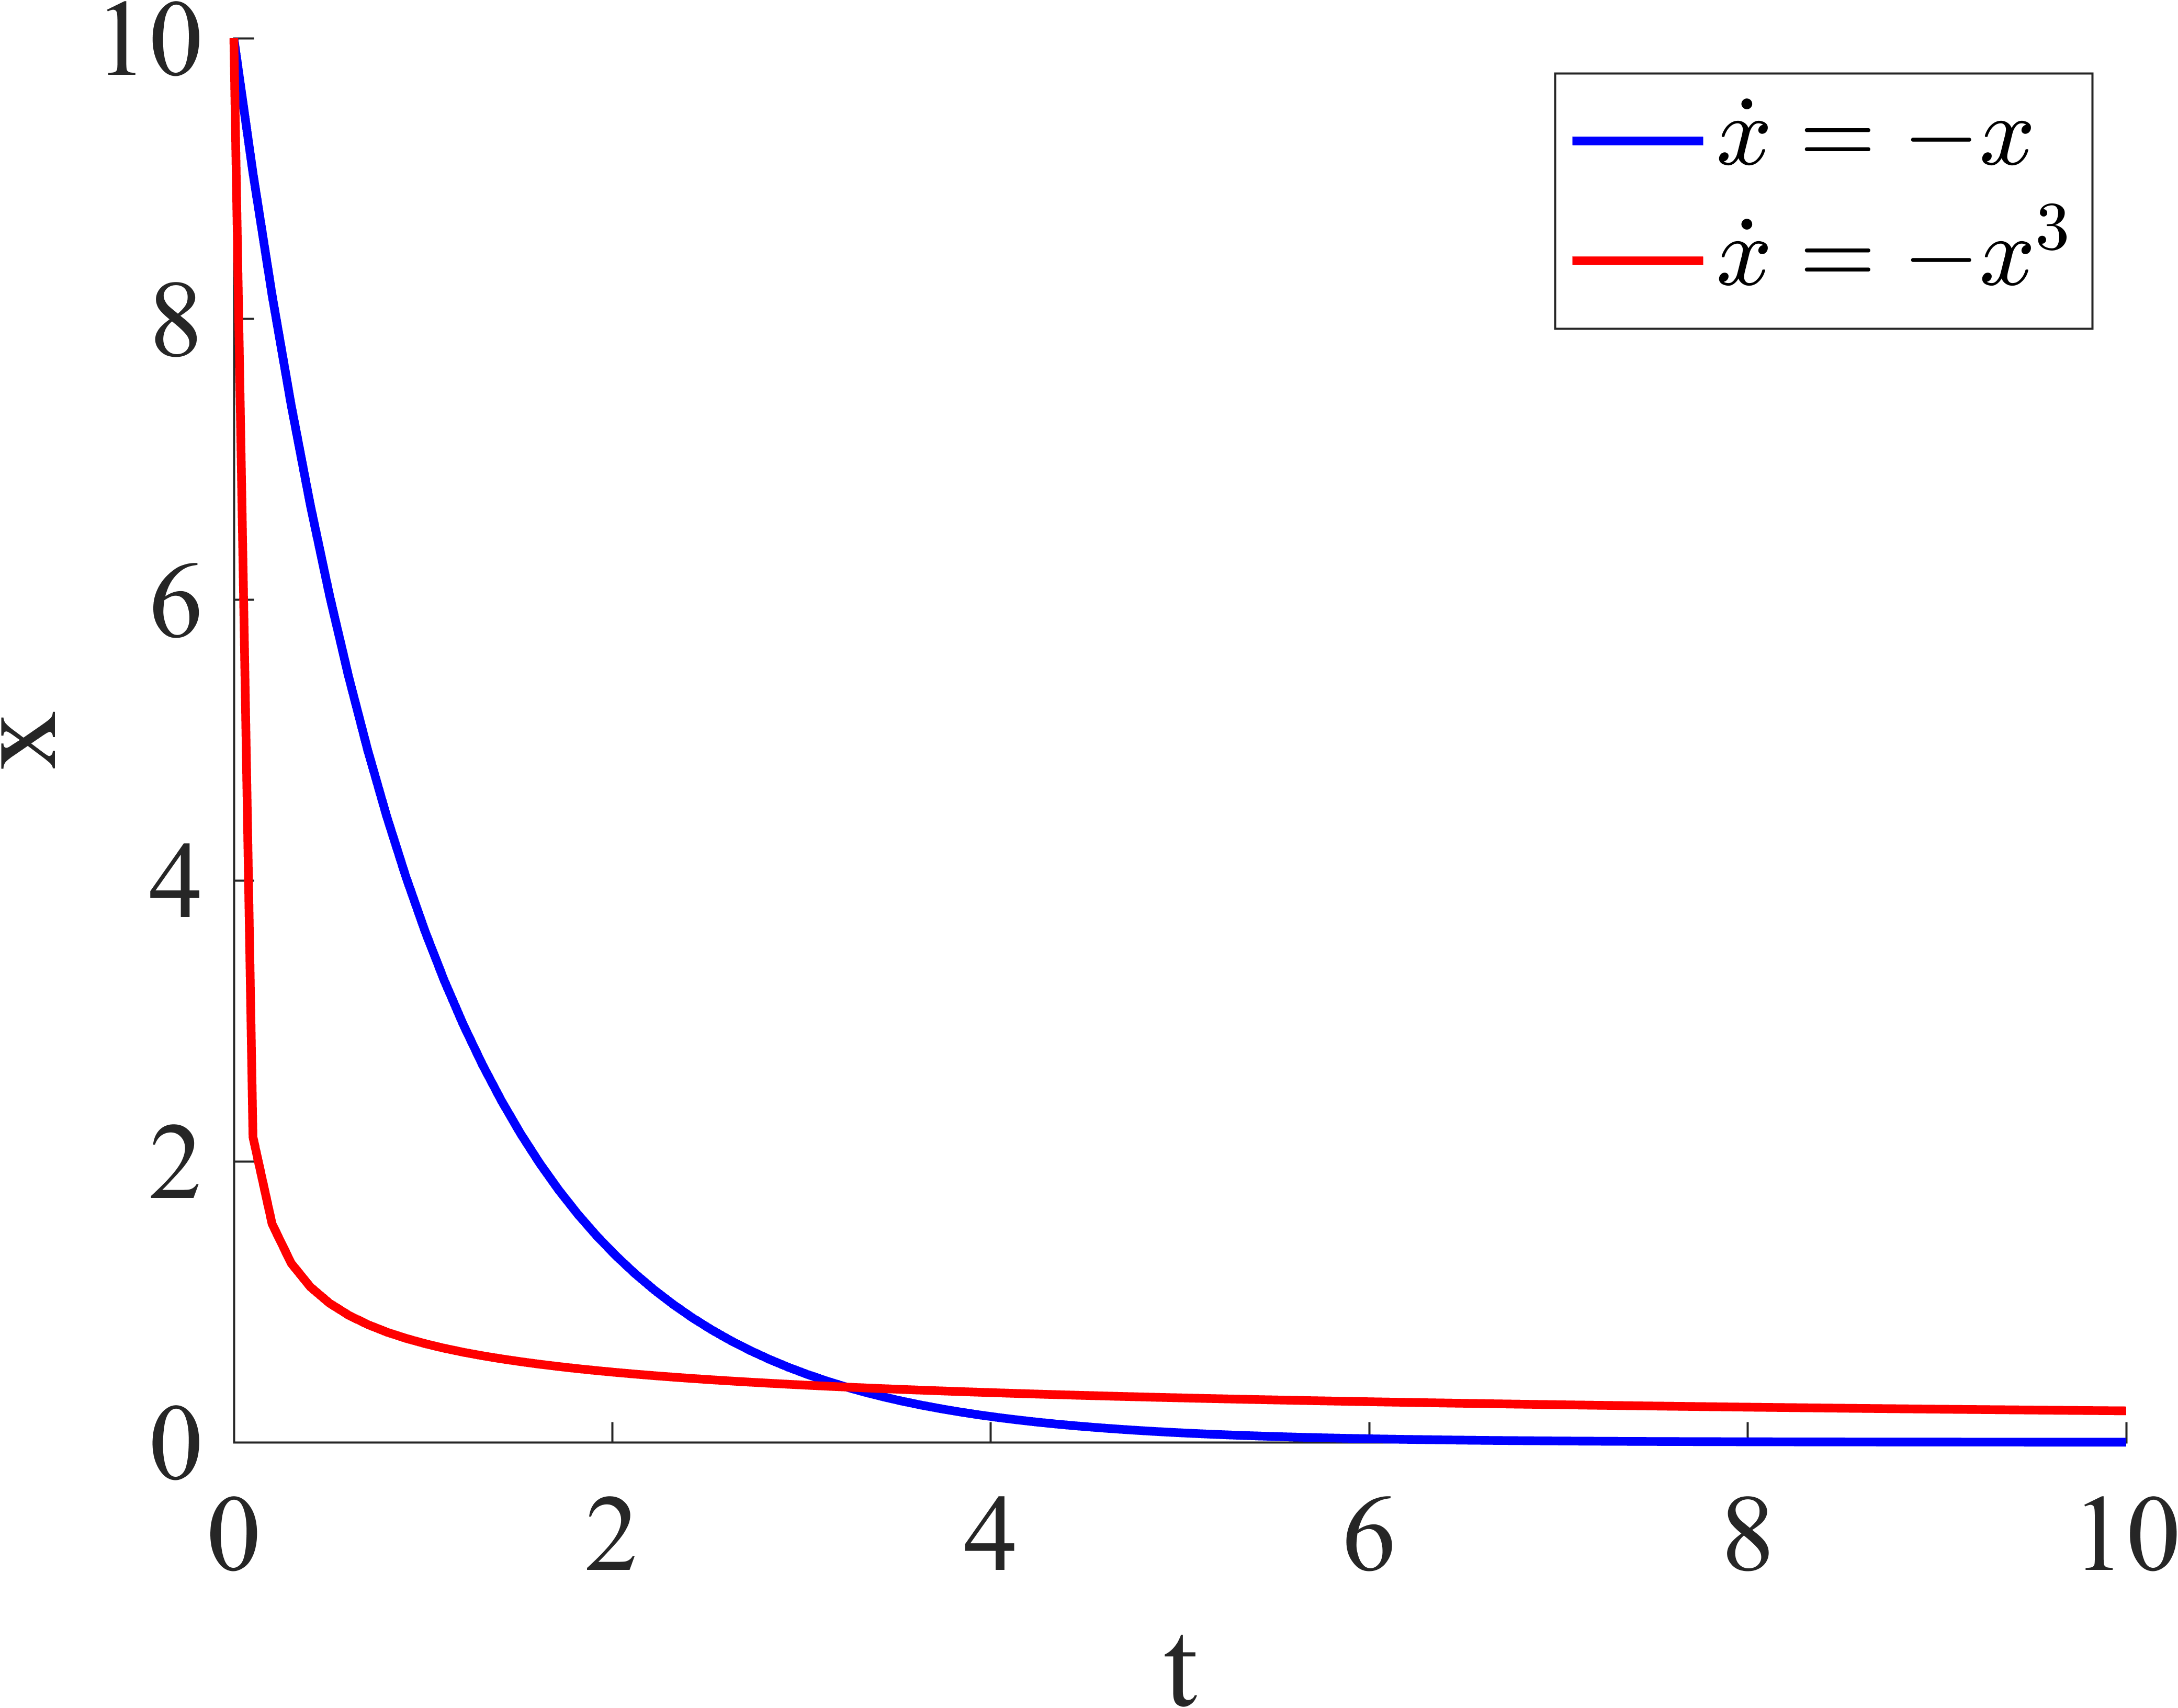
\includegraphics[width=10cm]{2_4_9_c}
\caption{Solution Plots}
\end{figure}
We see here that the decay for $\dot{x} = -x^3$ is much slower than for $\dot{x} = -x$ as $t \rightarrow \infty$. So the system reaches the equilibrium fixed point much more slowly.

\section*{Problem 8 Part 1.3}
Here I plot the flow for $ r = 1$. As we see here, the population always steadily approaches the carrying capacity without oscillations in a simple way because ODEs constrain the geometry of the flow. This is because ODEs are well-defined and finite throughout the entire state space. This means that the trajectories must be continuous and cannot cross. Furthermore, ODEs that are Lipschitz continuous (like $\frac{d}{d \tau} N(\tau) = N(\tau)(1- N(\tau))$) also must have unique trajectories that cannot merge or branch in finite time.


\begin{figure}[h]
\centering
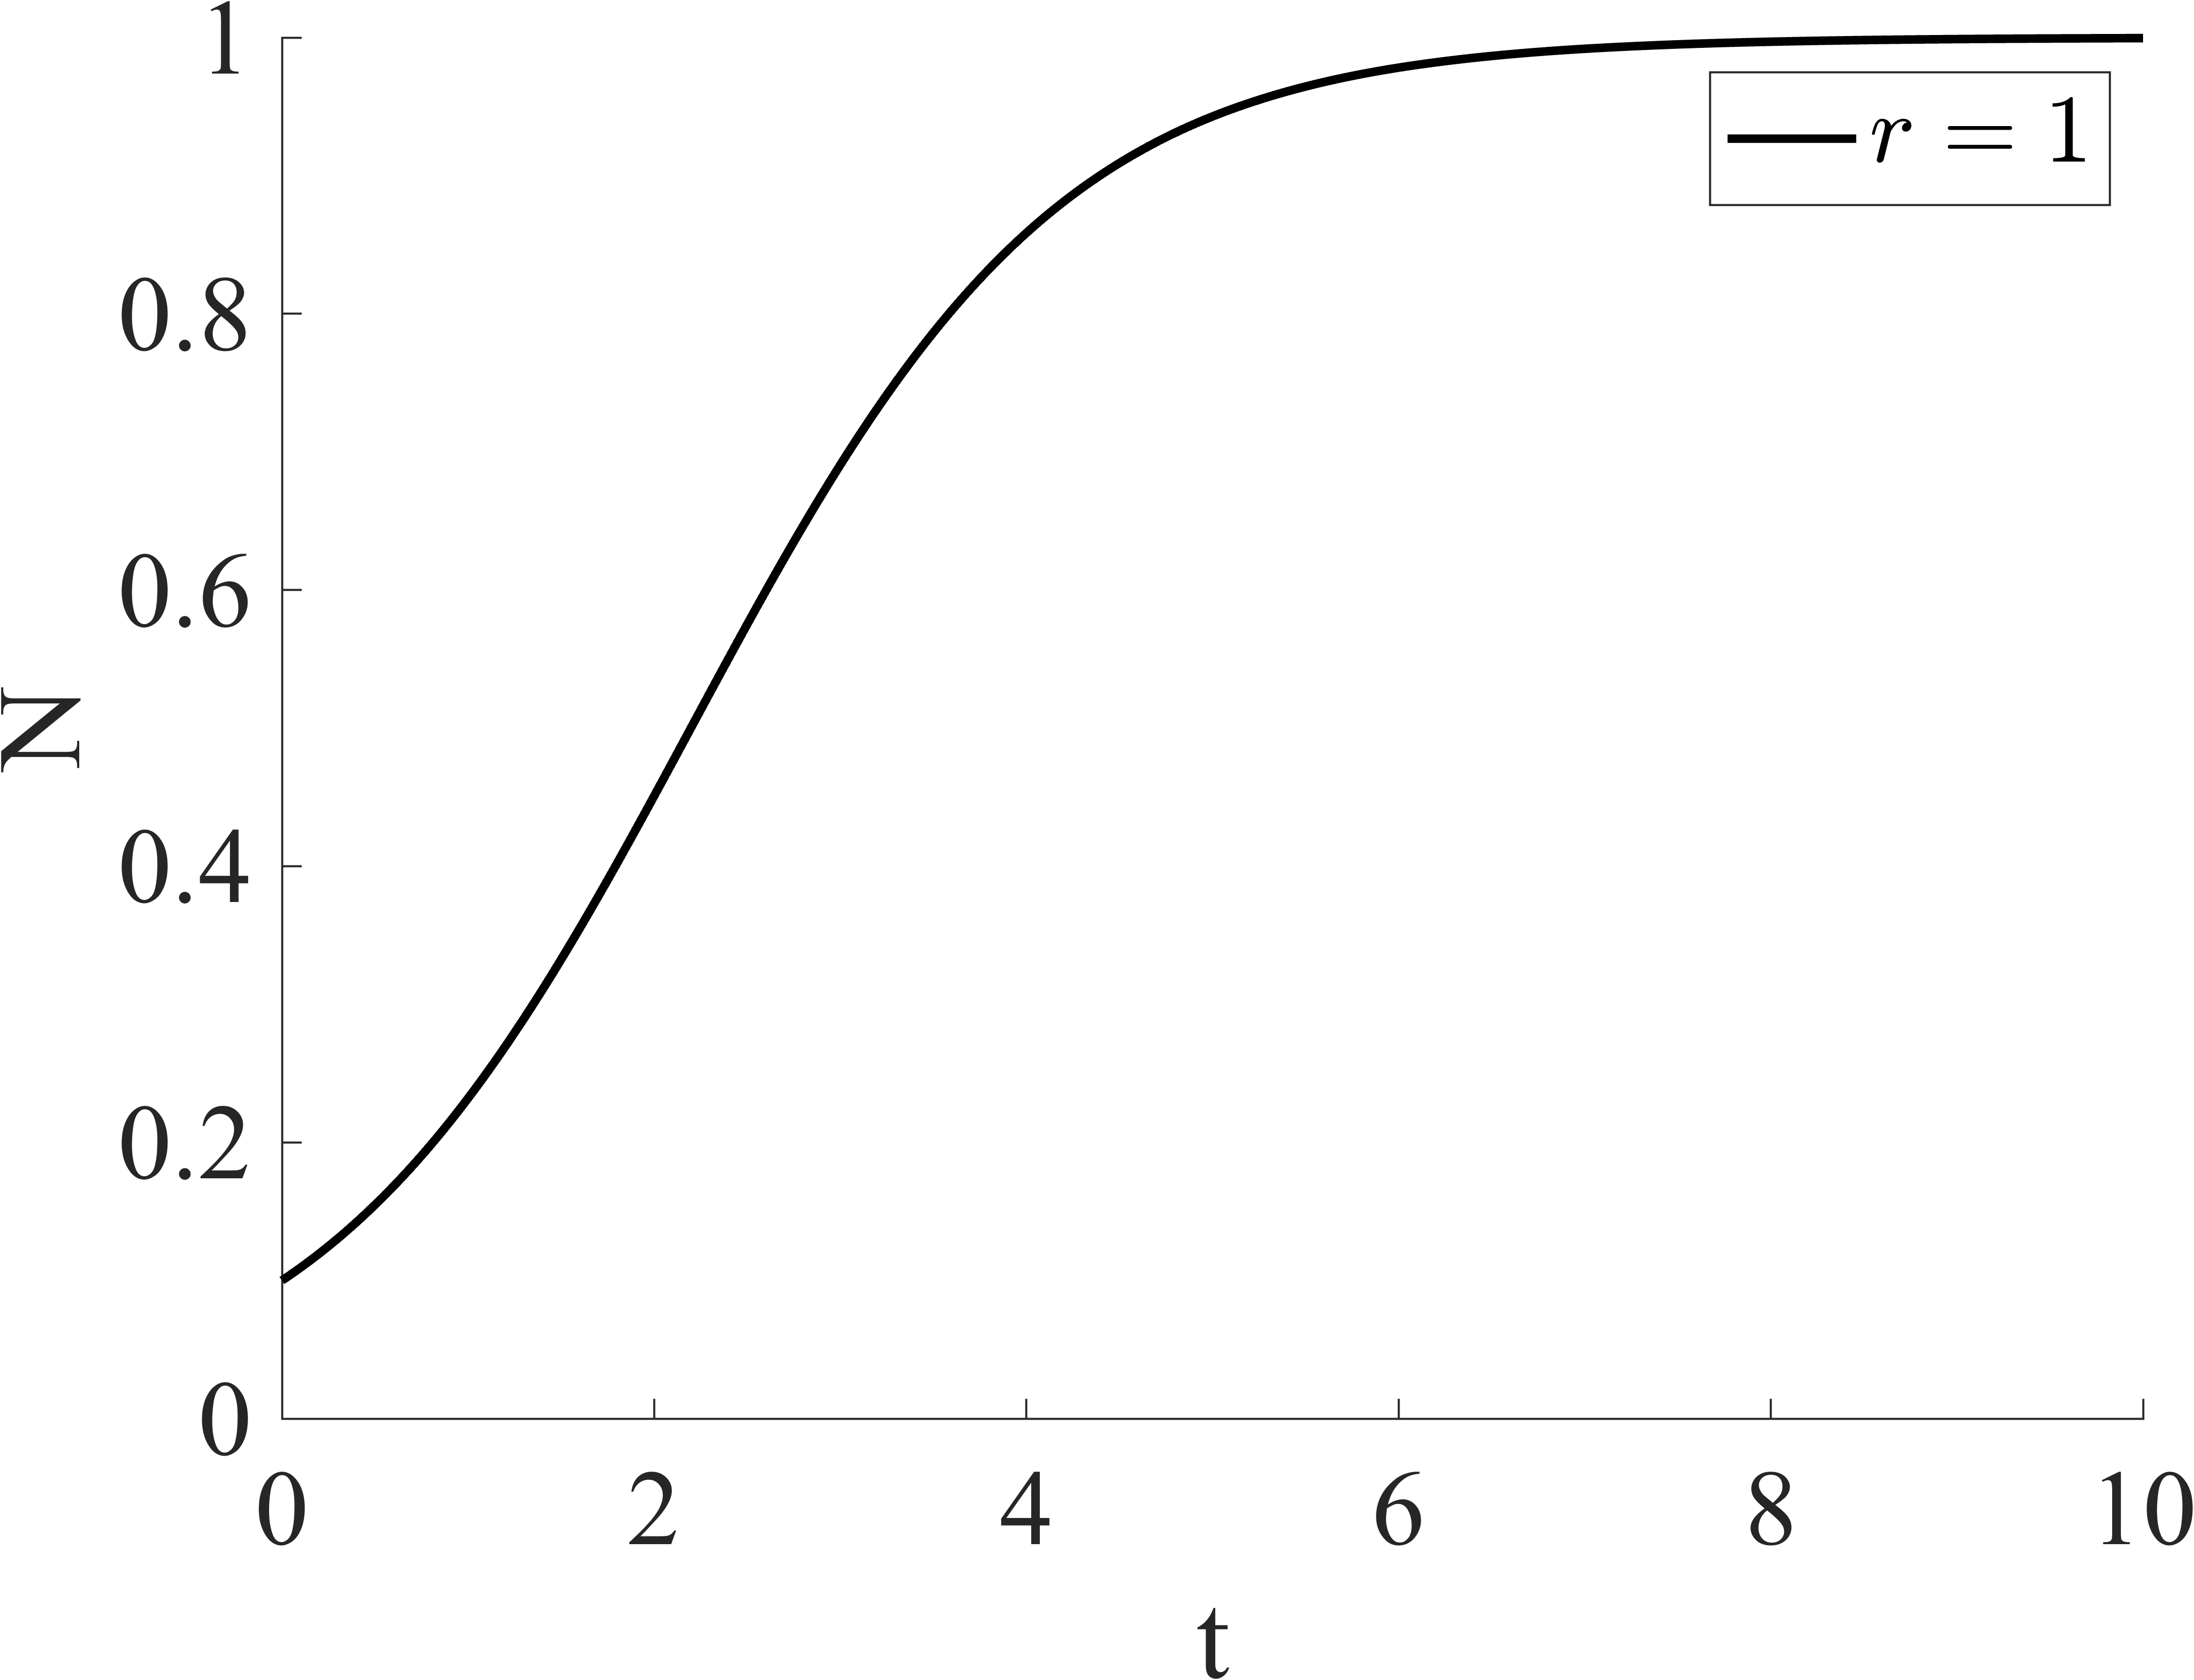
\includegraphics[width=10cm]{8_p1_3}x
\caption{Solution Plots}
\end{figure}


\section*{Problem 8 Part 2.3}
Here I plot cobweb plots for two sets of $r$, one for $ r = 2, 2.5, 3$ and one for $r = 3.25, 3.5, 3.57$. I do the plots for two initial conditions, $N_0 = 0.05$ and $N_0 = 0.4$.
\begin{figure}[h]
\centering
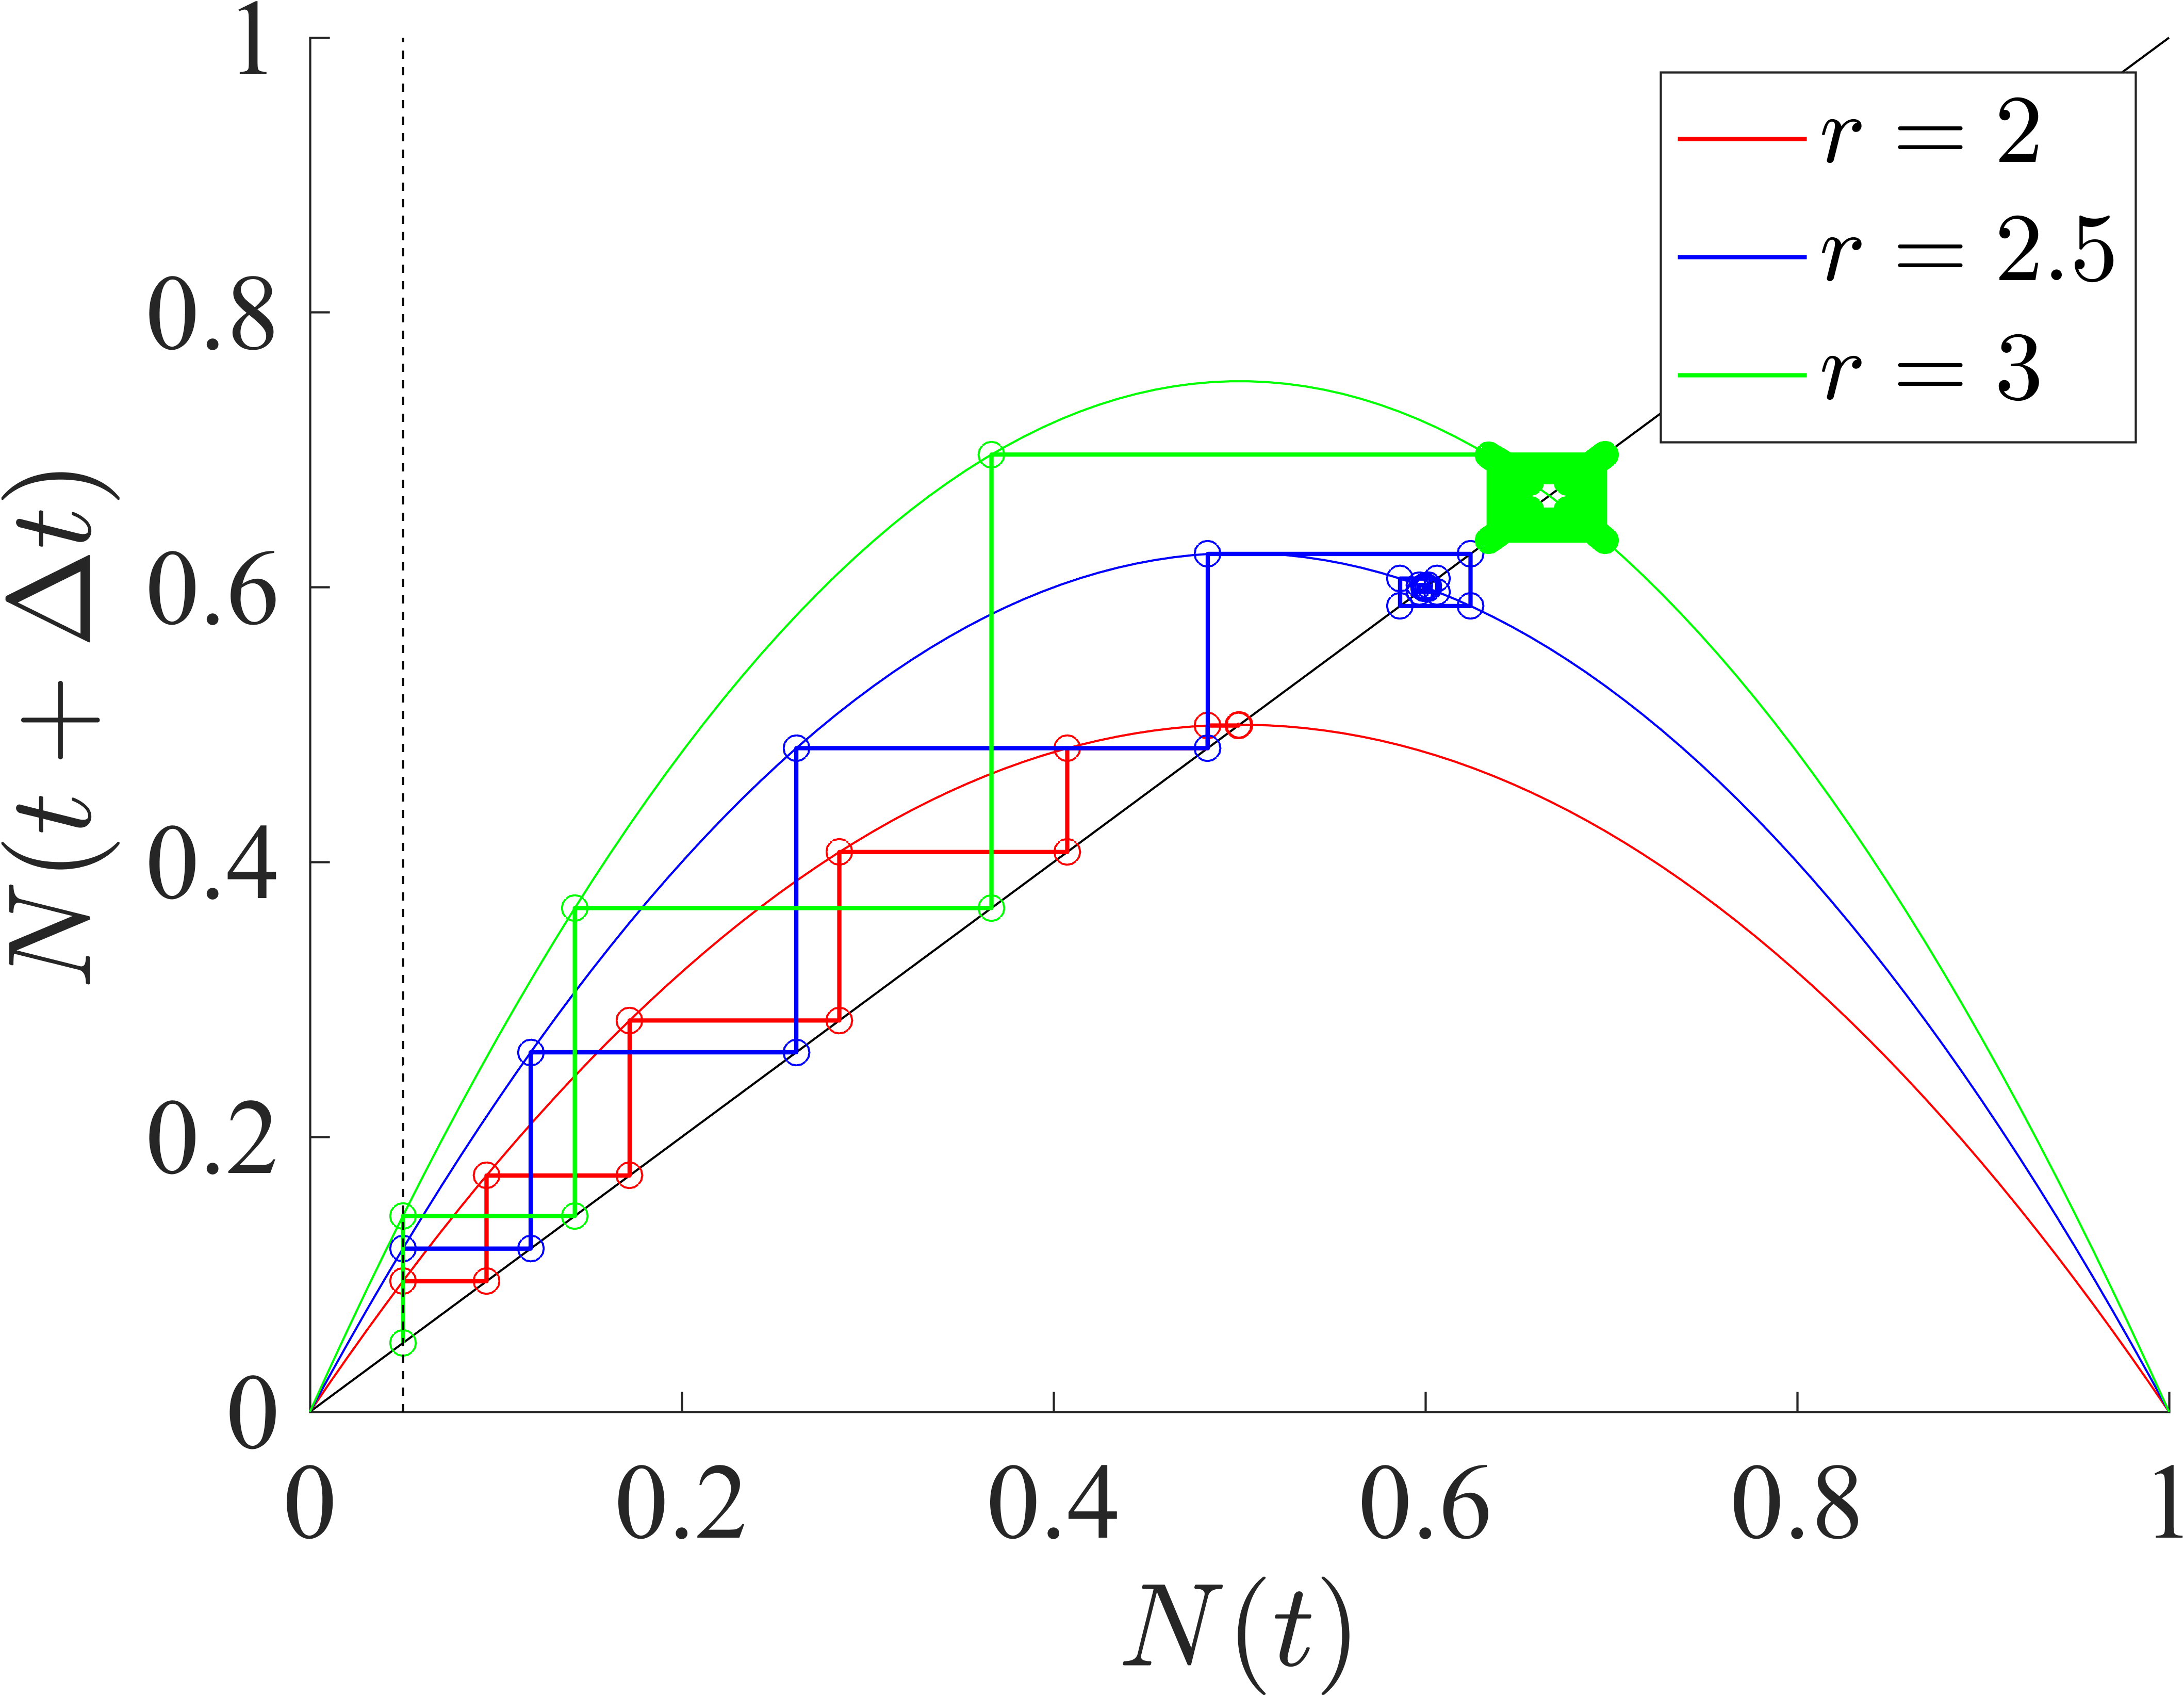
\includegraphics[width=10cm]{8_p2_3_1_r0_05}
\caption{Cobweb Plots $N_0 = 0.05$}
\end{figure}

\begin{figure}[H]
\centering
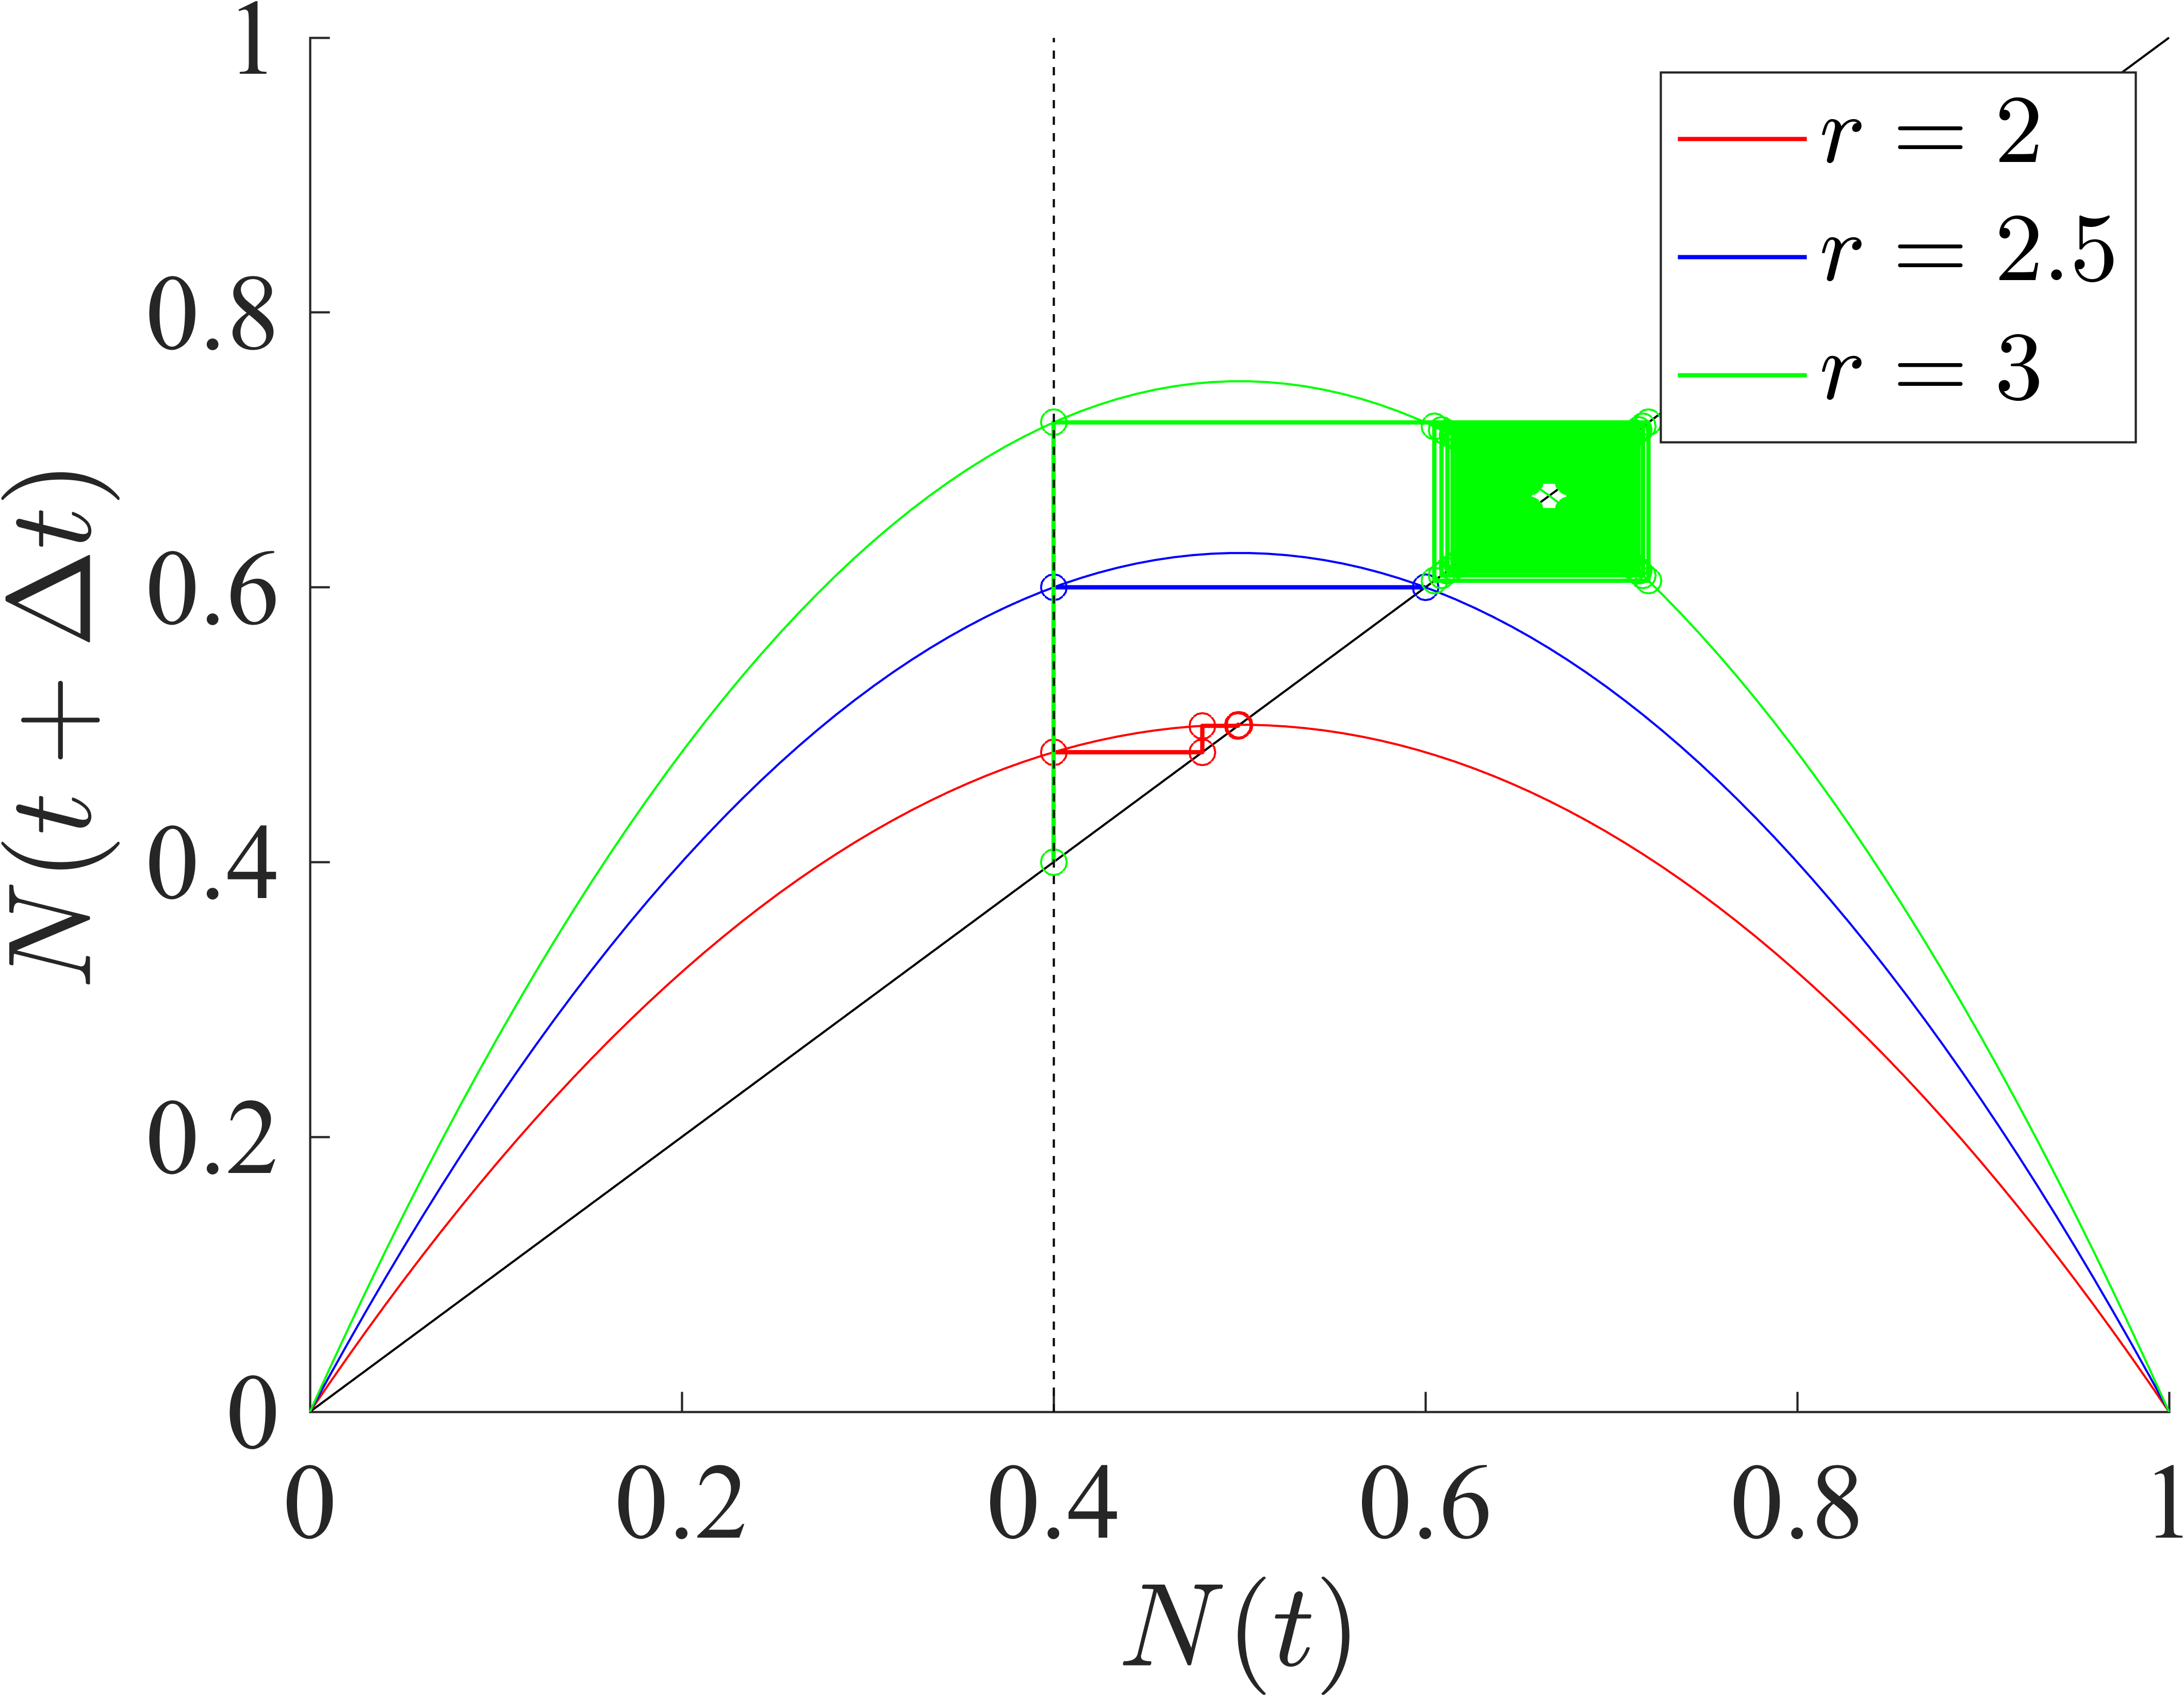
\includegraphics[width=10cm]{8_p2_3_1_r0_4}
\caption{Cobweb Plots $N_0 = 0.4$}
\end{figure}


We see in the figures above that for $r = 2$ and $r = 2.5$, the logistic map approaches a stable solution for different initial conditions. However, for $r = 2.5$, the approach is not monotonic. When $r = 3$, the solution appears to approach a steady oscillation.

Now I plot cobweb plots for $r = 3.25, 3.5, 3.57$.

\begin{figure}[h]
\centering
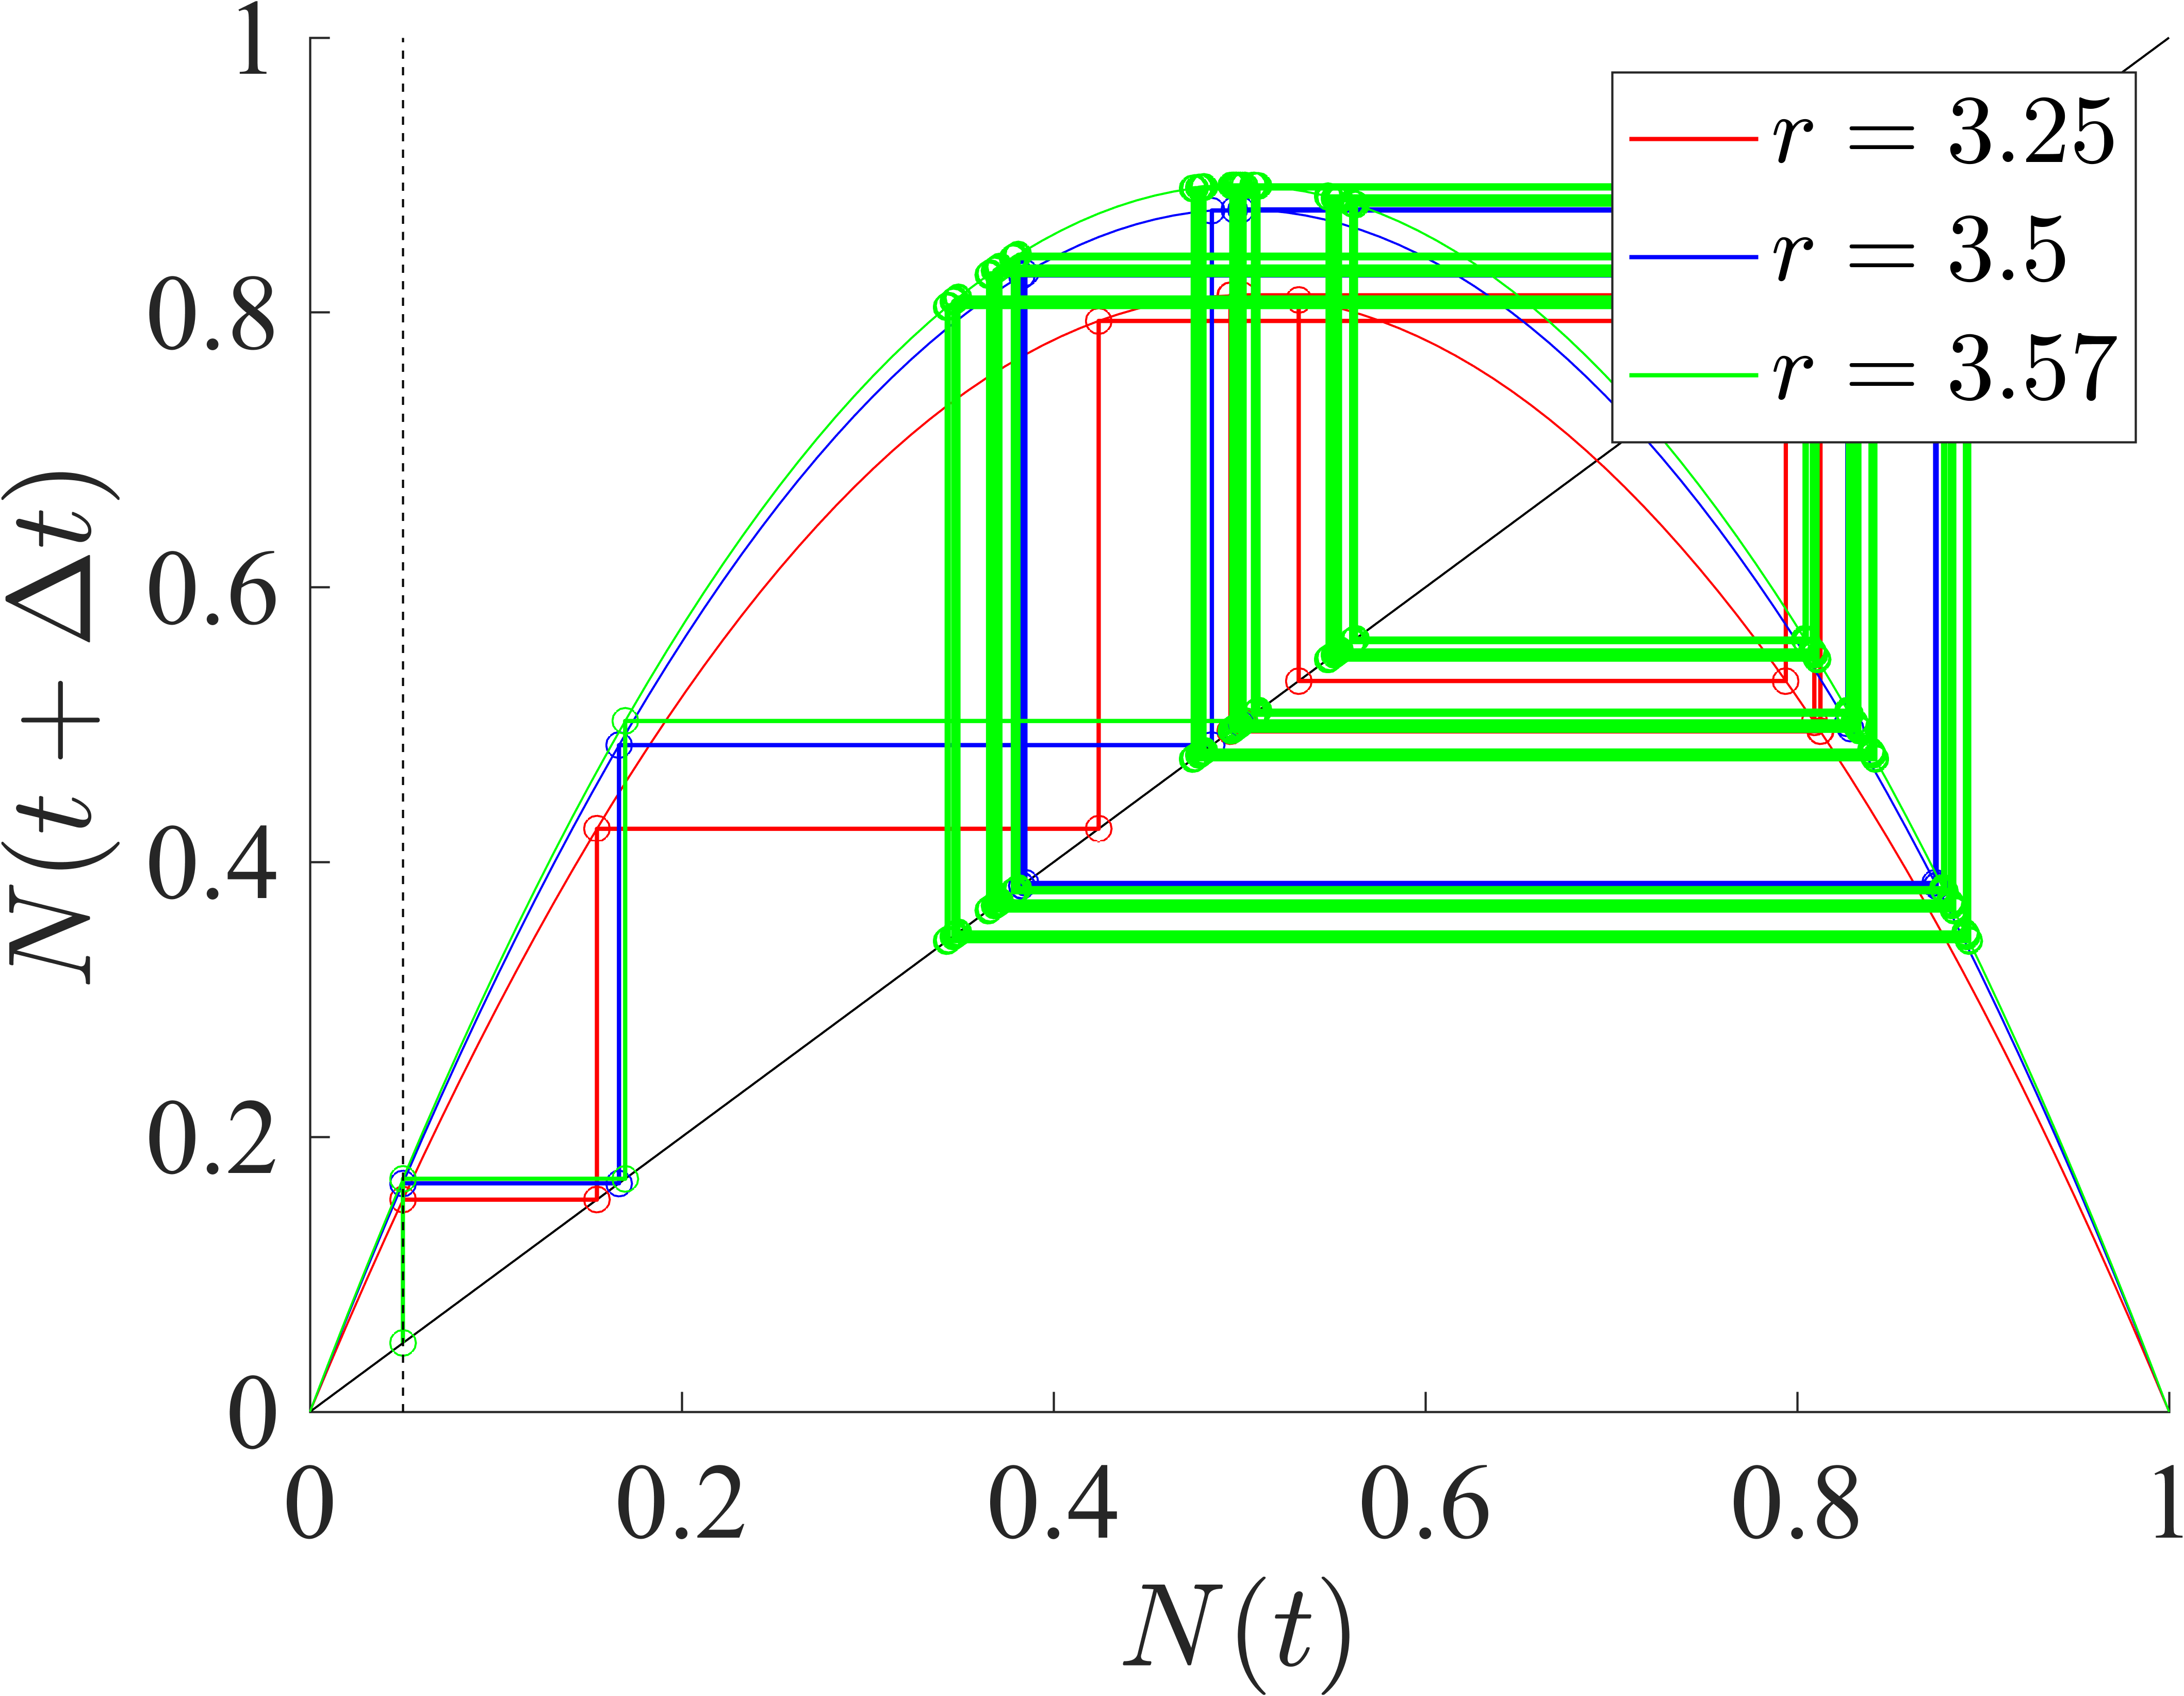
\includegraphics[width=10cm]{8_p2_3_2_r0_05}
\caption{Cobweb Plots $N_0 = 0.05$}
\end{figure}


\begin{figure}[H]
\centering
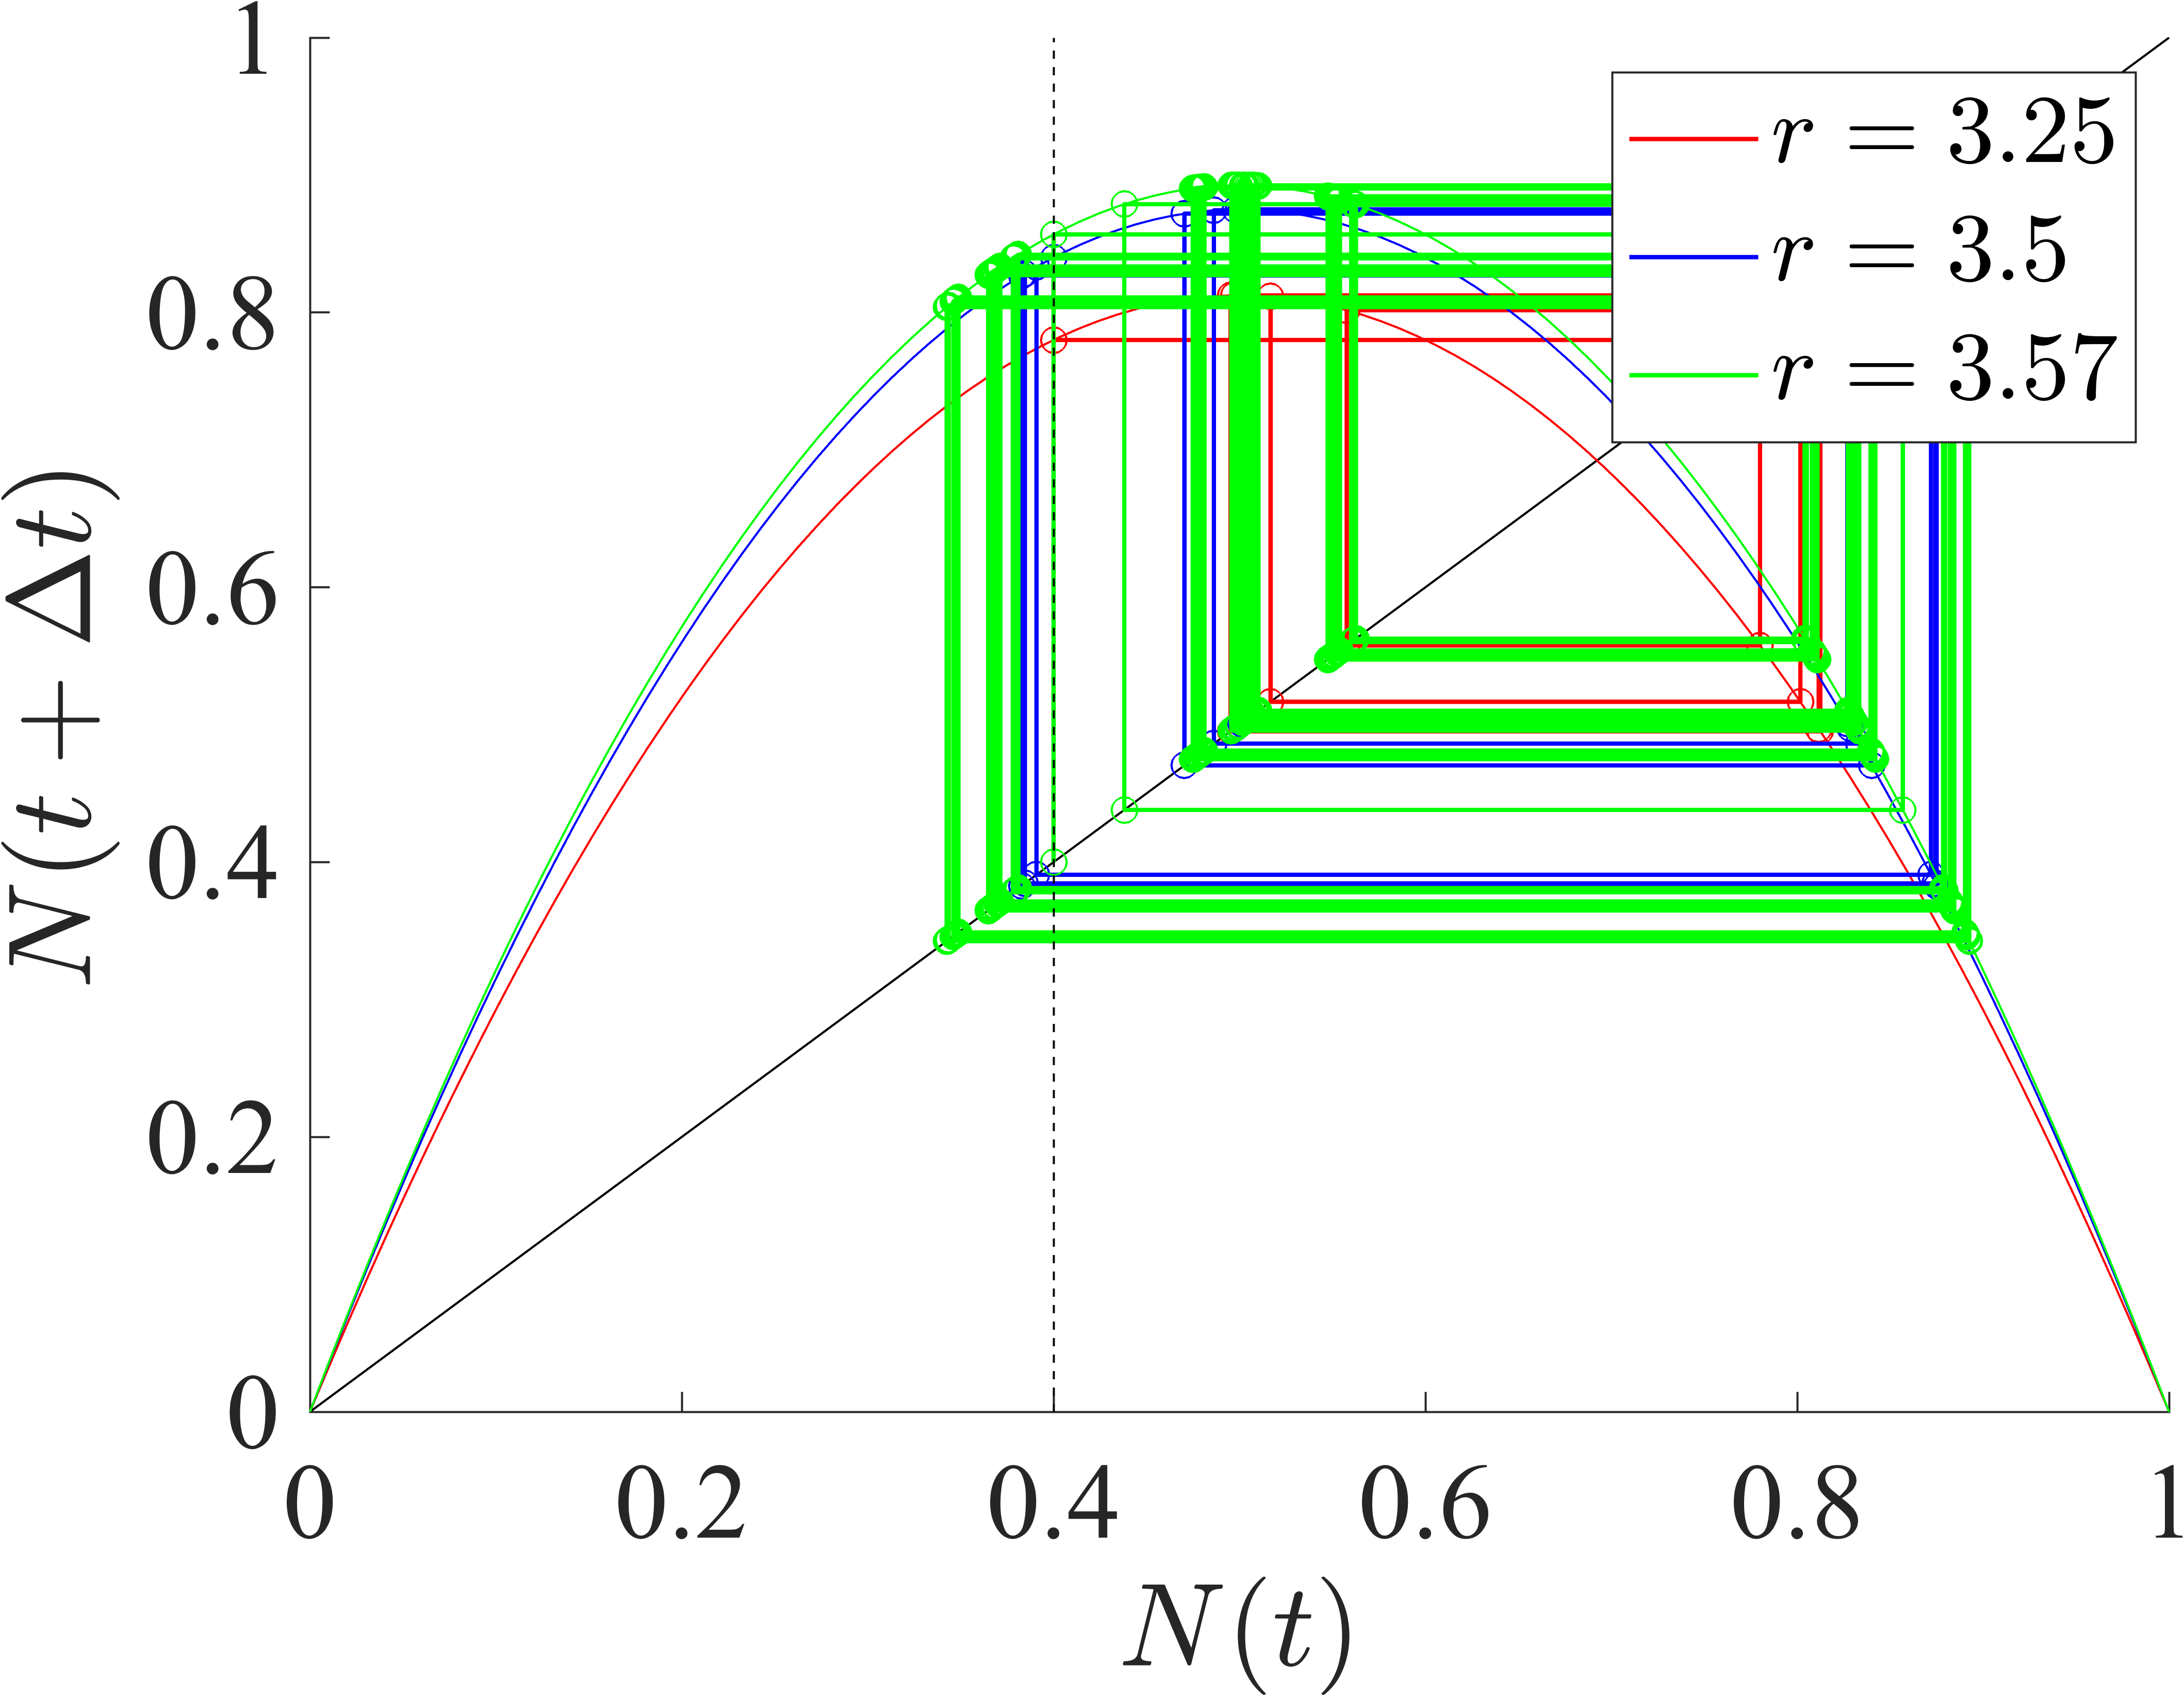
\includegraphics[width=10cm]{8_p2_3_2_r0_4}
\caption{Cobweb Plots $N_0 = 0.4$}
\end{figure}

We see here that the solutions with $r = 3.25$ and $r = 3.5$ appear to have steady oscillations, while the logistic map with $r = 3.57$ appears to be chaotic. We can confirm these behaviors and approximate the period of the oscillations by plotting $N(t)$ versus $t$ for $t$ ranging from 1 to 32.

\begin{figure}[H]
\centering
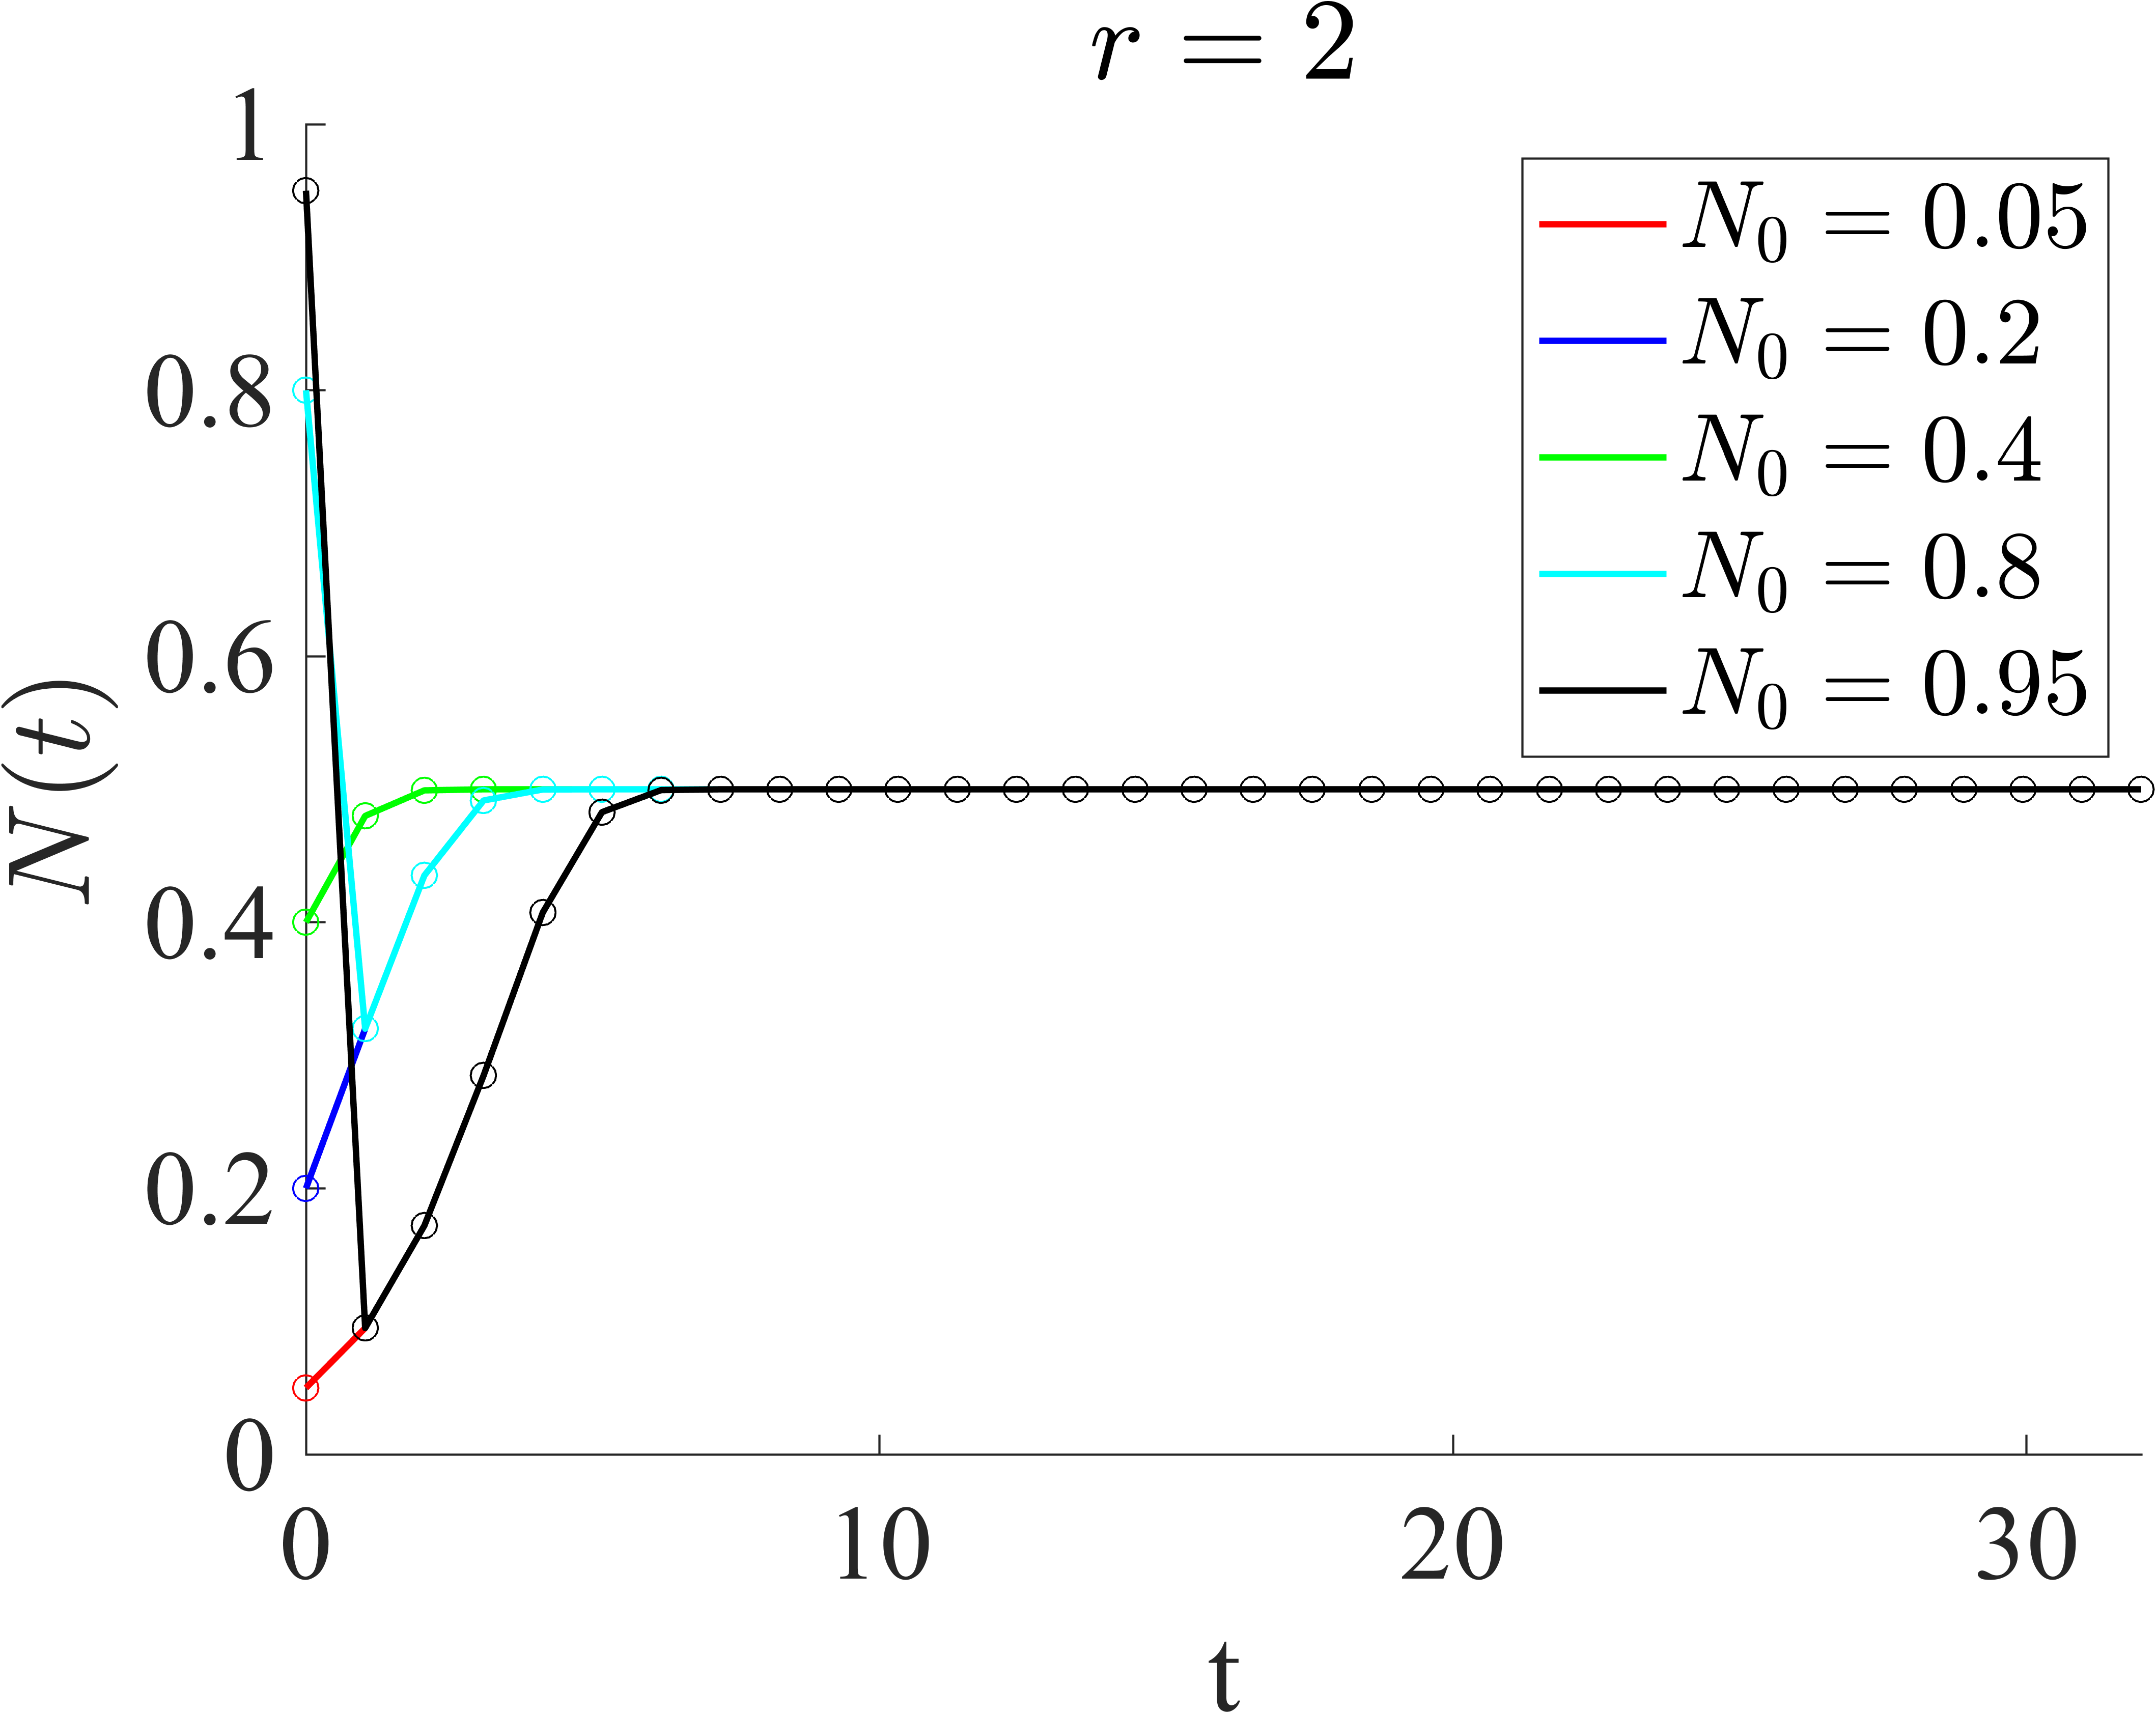
\includegraphics[width=10cm]{Logistic_map_r_2}
\caption{Logistic Map Solution Plot}
\end{figure}
As expected, for $r = 2$, the solution approaches a steady state regardless of initial condition. Even here, however, the approach for $N_0 = 0.95$ and $N_0=0.8$ are not monotonic because $N$ decreases below the stable value before going back up. Thus, $N(t)$ does not approach the fixed point monotonically for some initial conditions.

\begin{figure}[H]
\centering
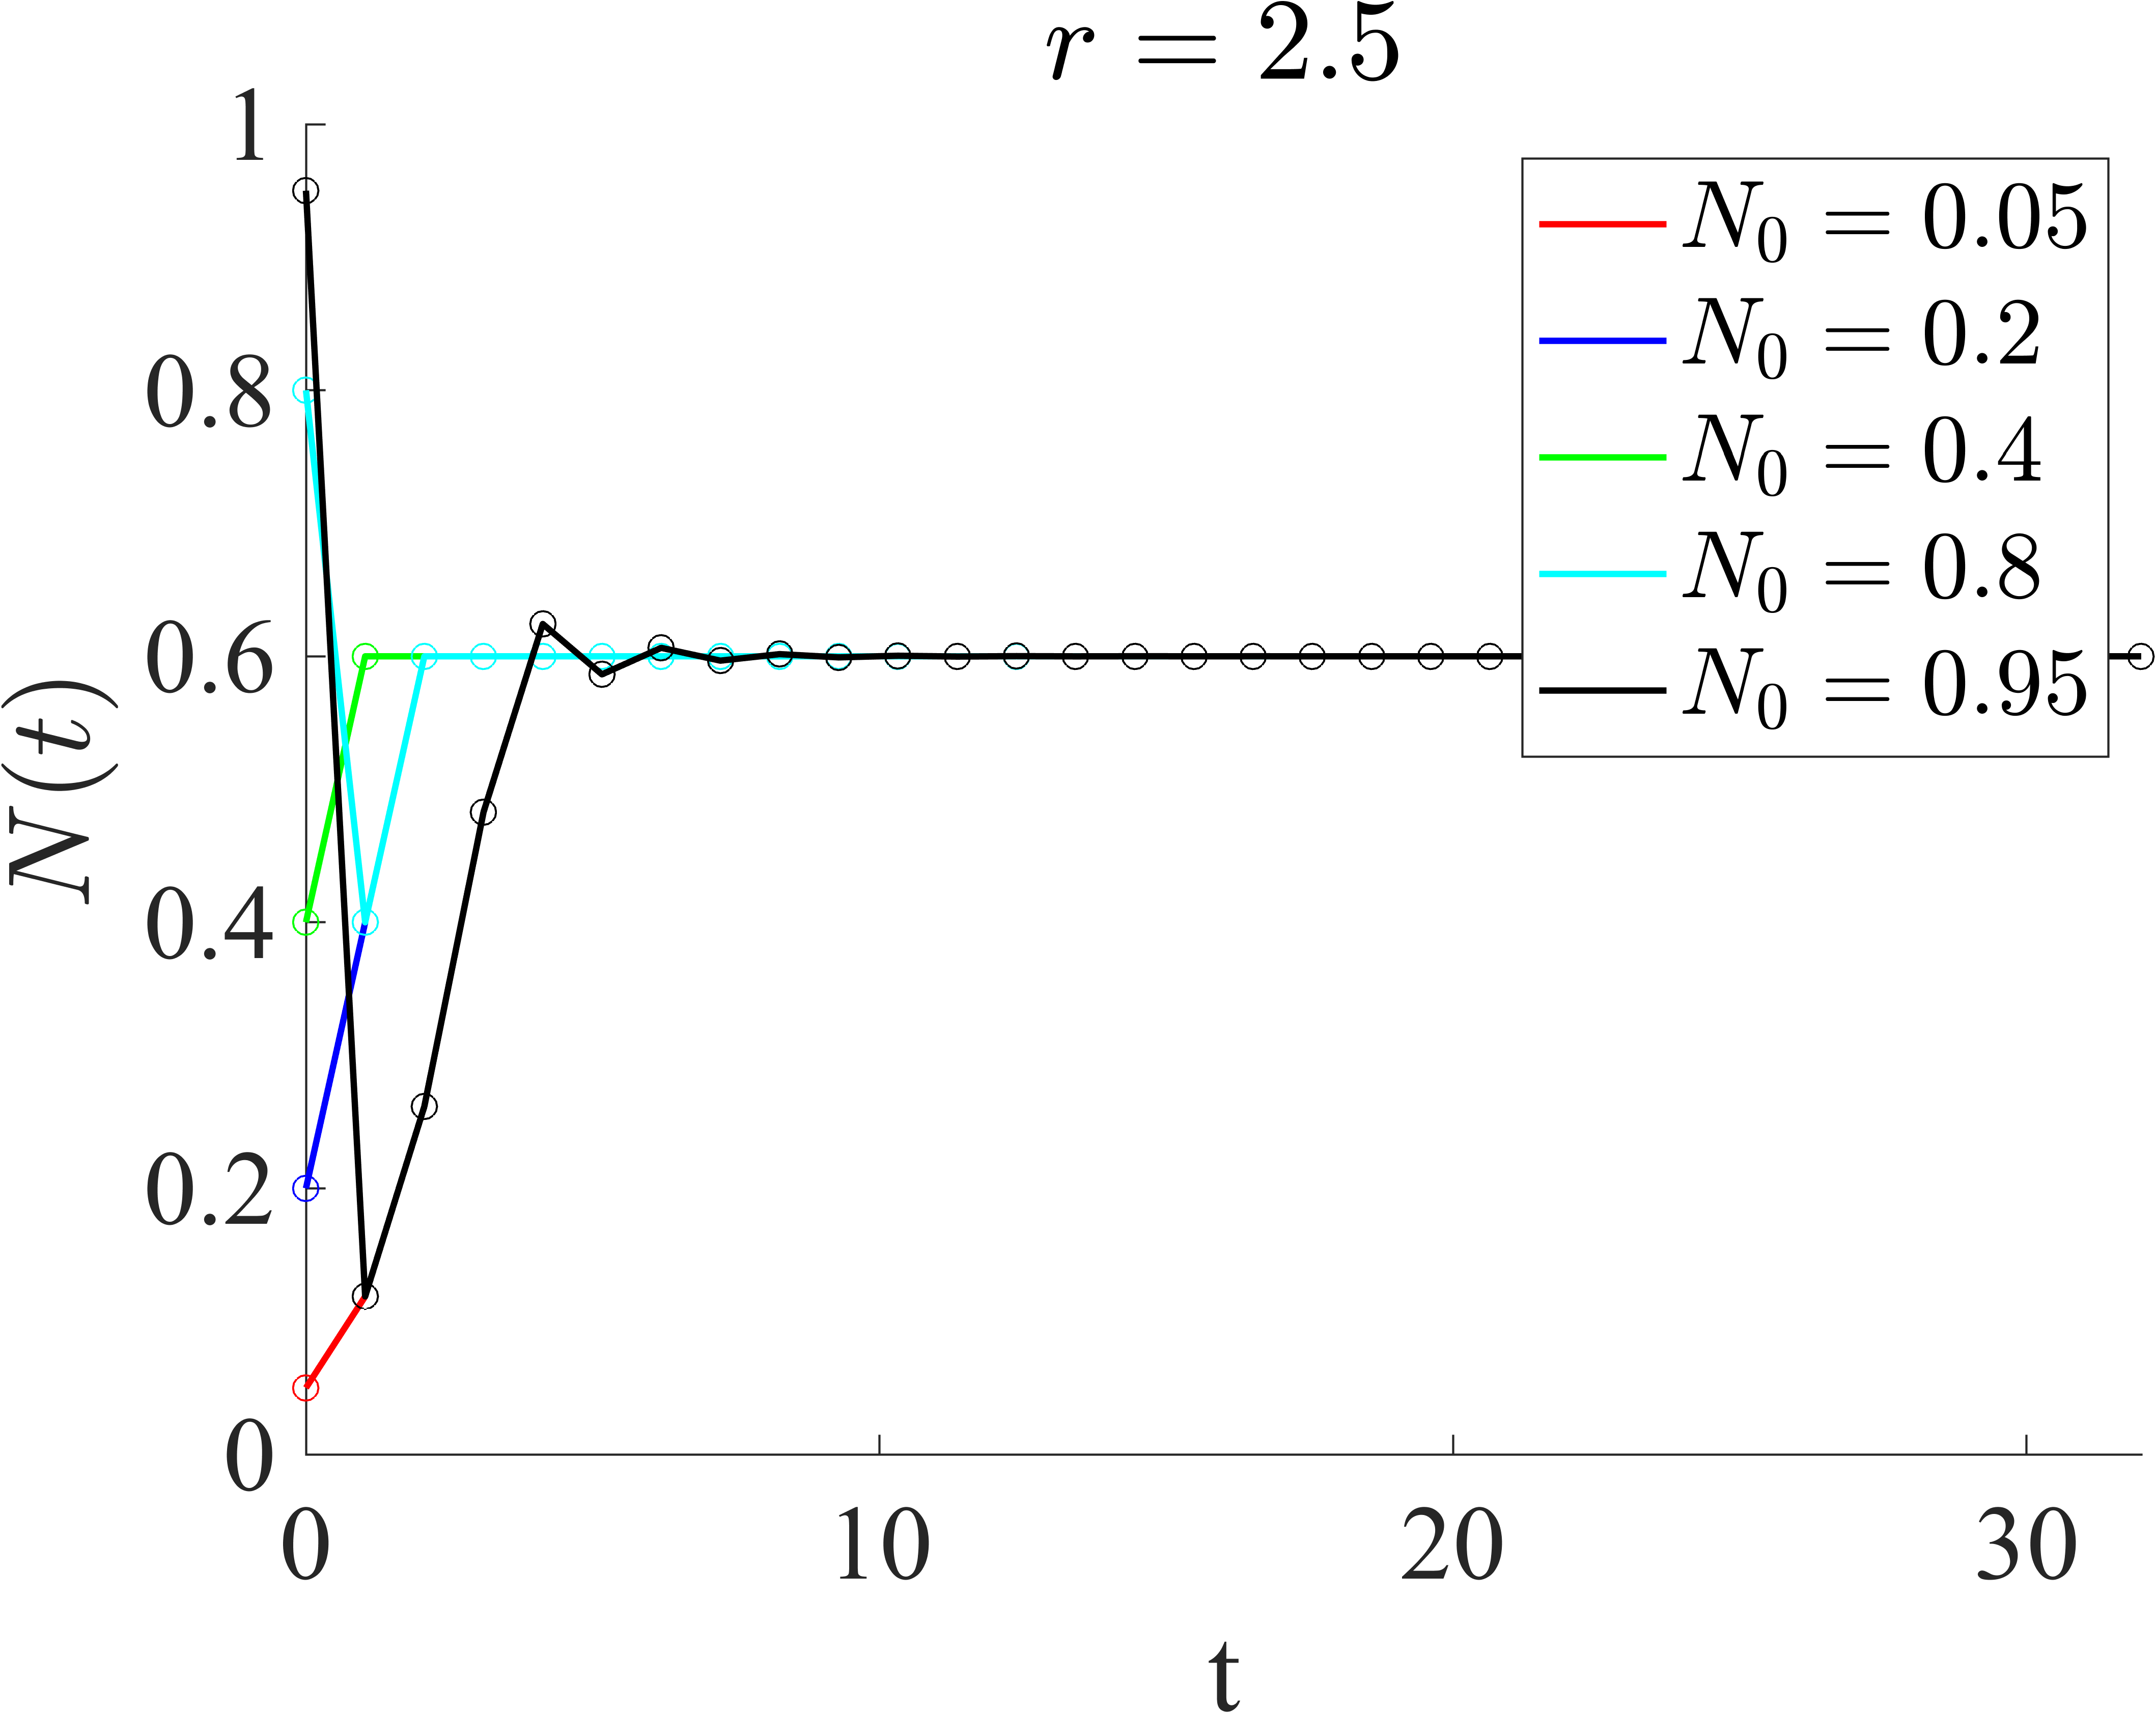
\includegraphics[width=10cm]{Logistic_map_r_2_5}
\caption{Logistic Map Solution Plot}
\end{figure}
The solutions similarly approach the fixed point for $r = 2.5$, but the approach is not always monotonic.

\begin{figure}[H]
\centering
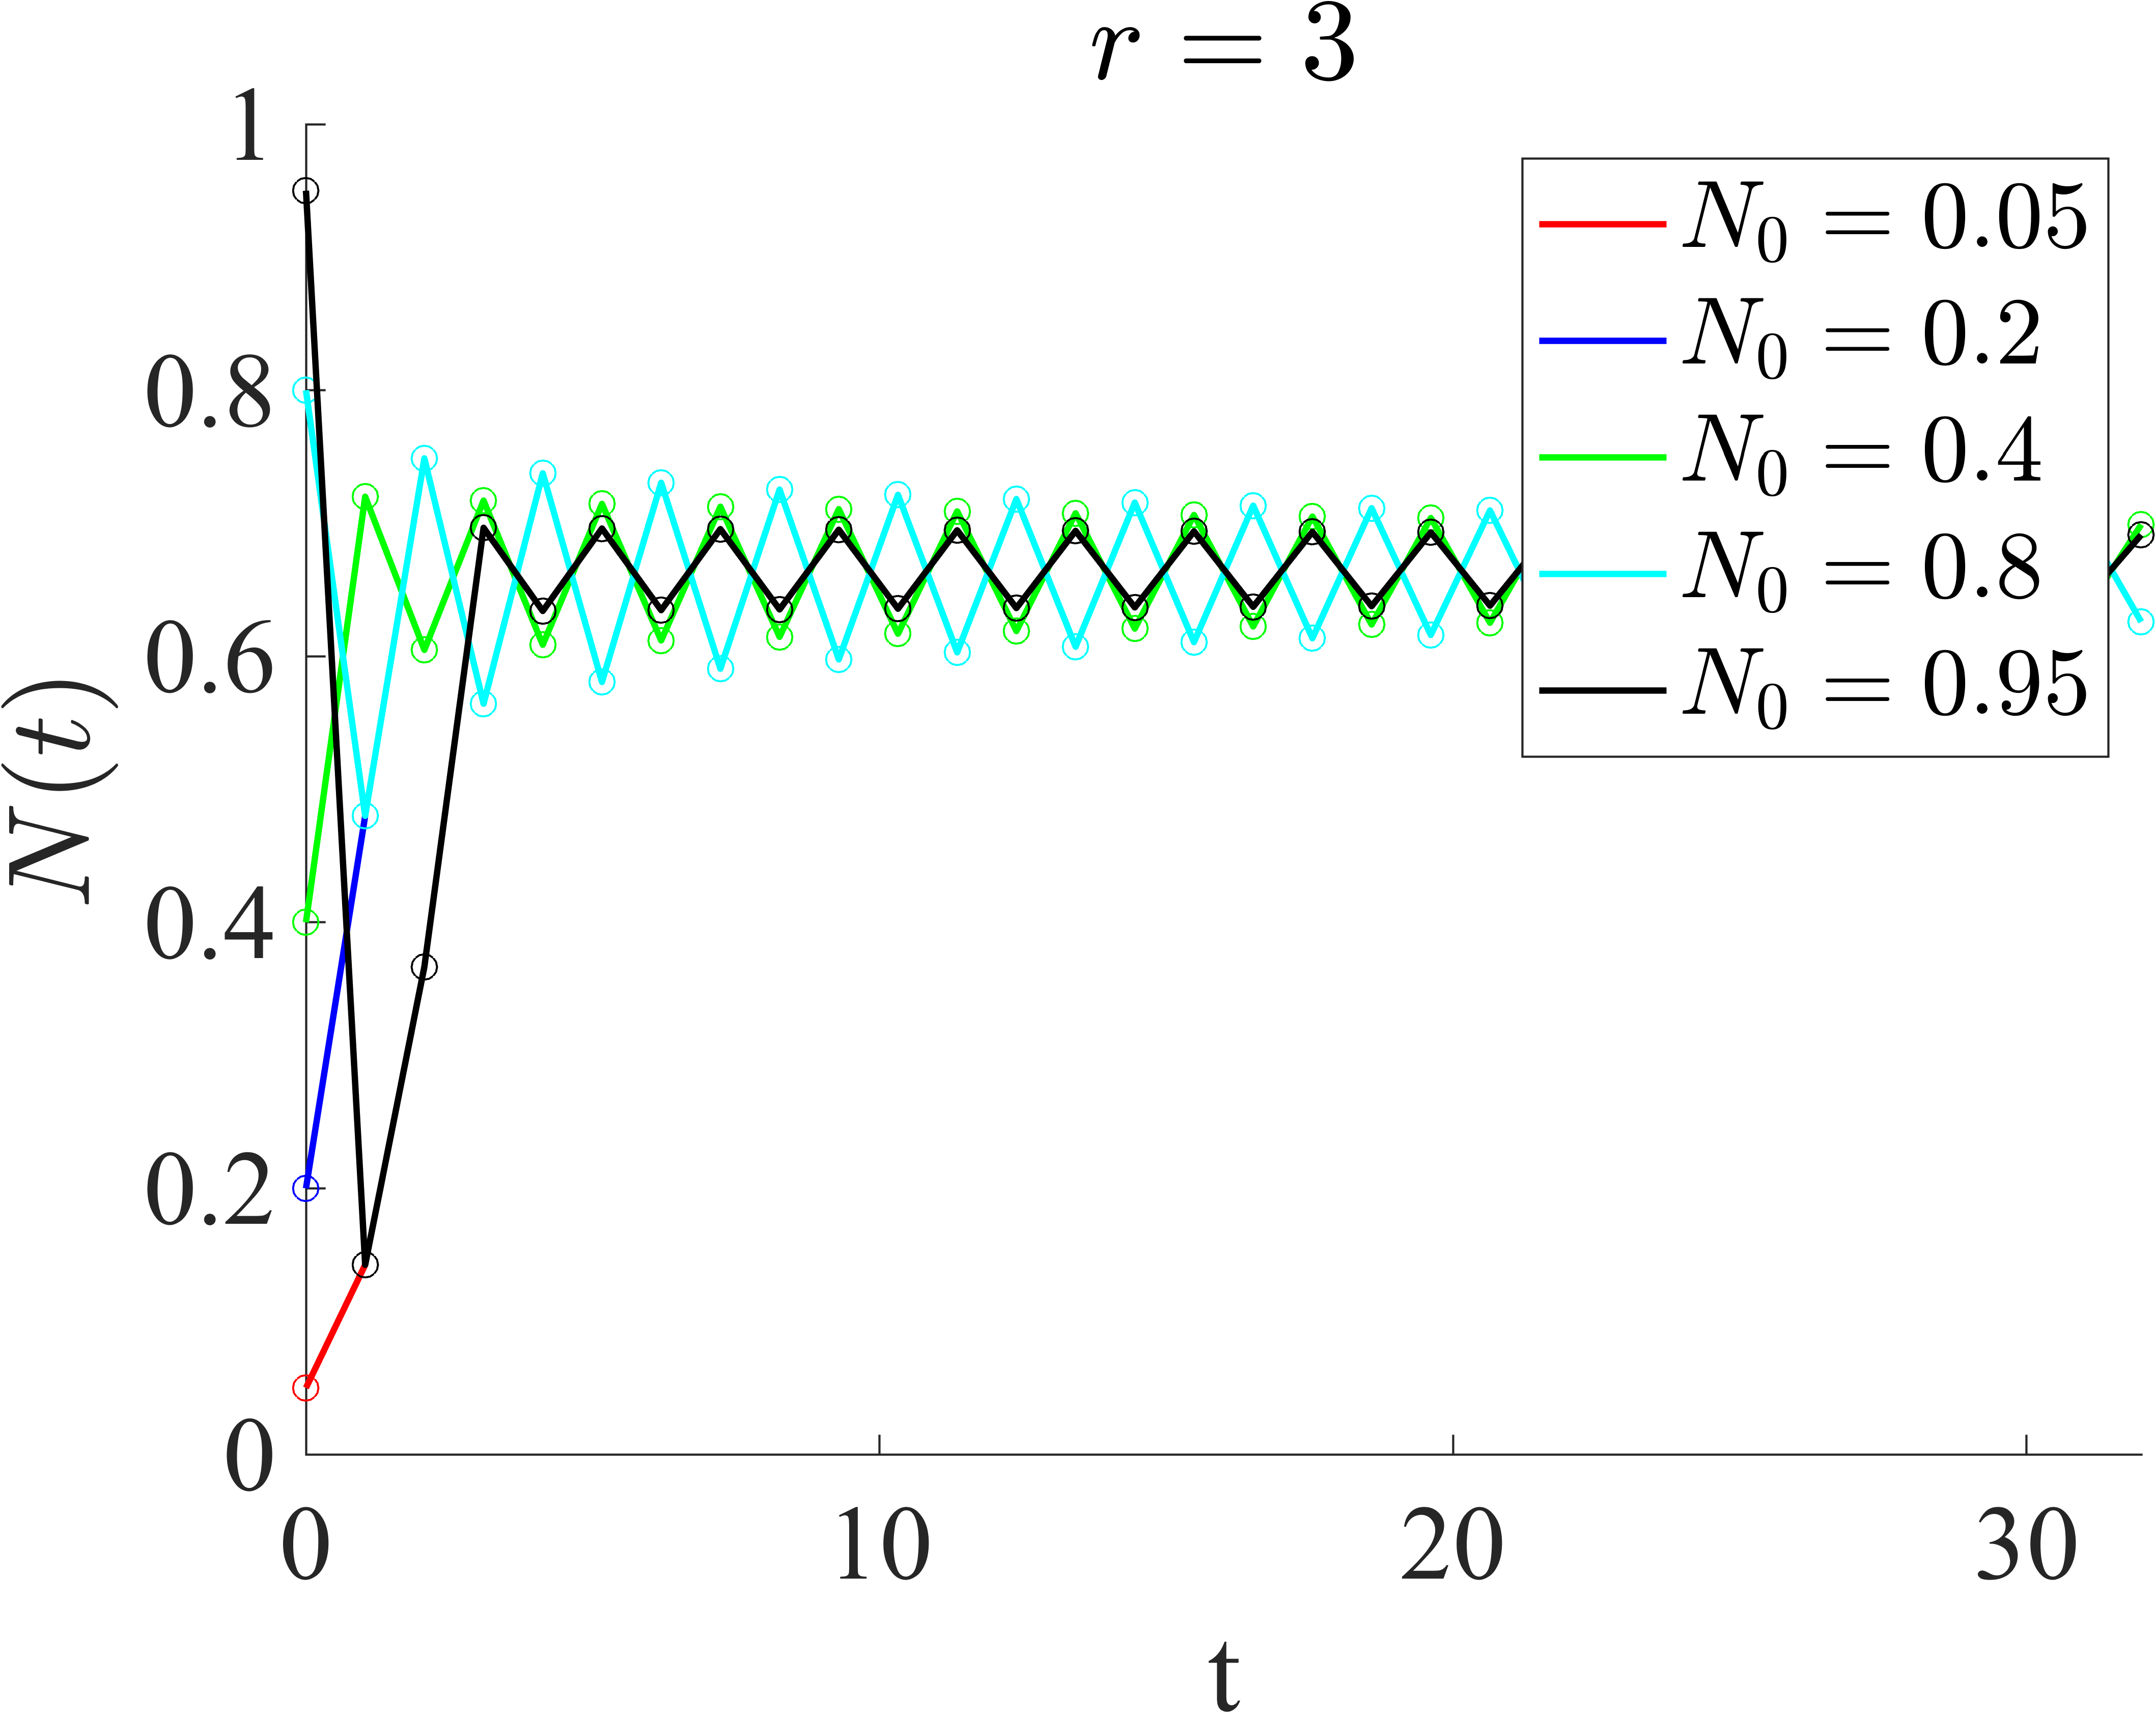
\includegraphics[width=10cm]{Logistic_map_r_3}
\caption{Logistic Map Solution Plot}
\end{figure}
With $r = 3$, the solutions appear to be in a stable oscillatory cycle of a period of 2 time steps.

\begin{figure}[H]
\centering
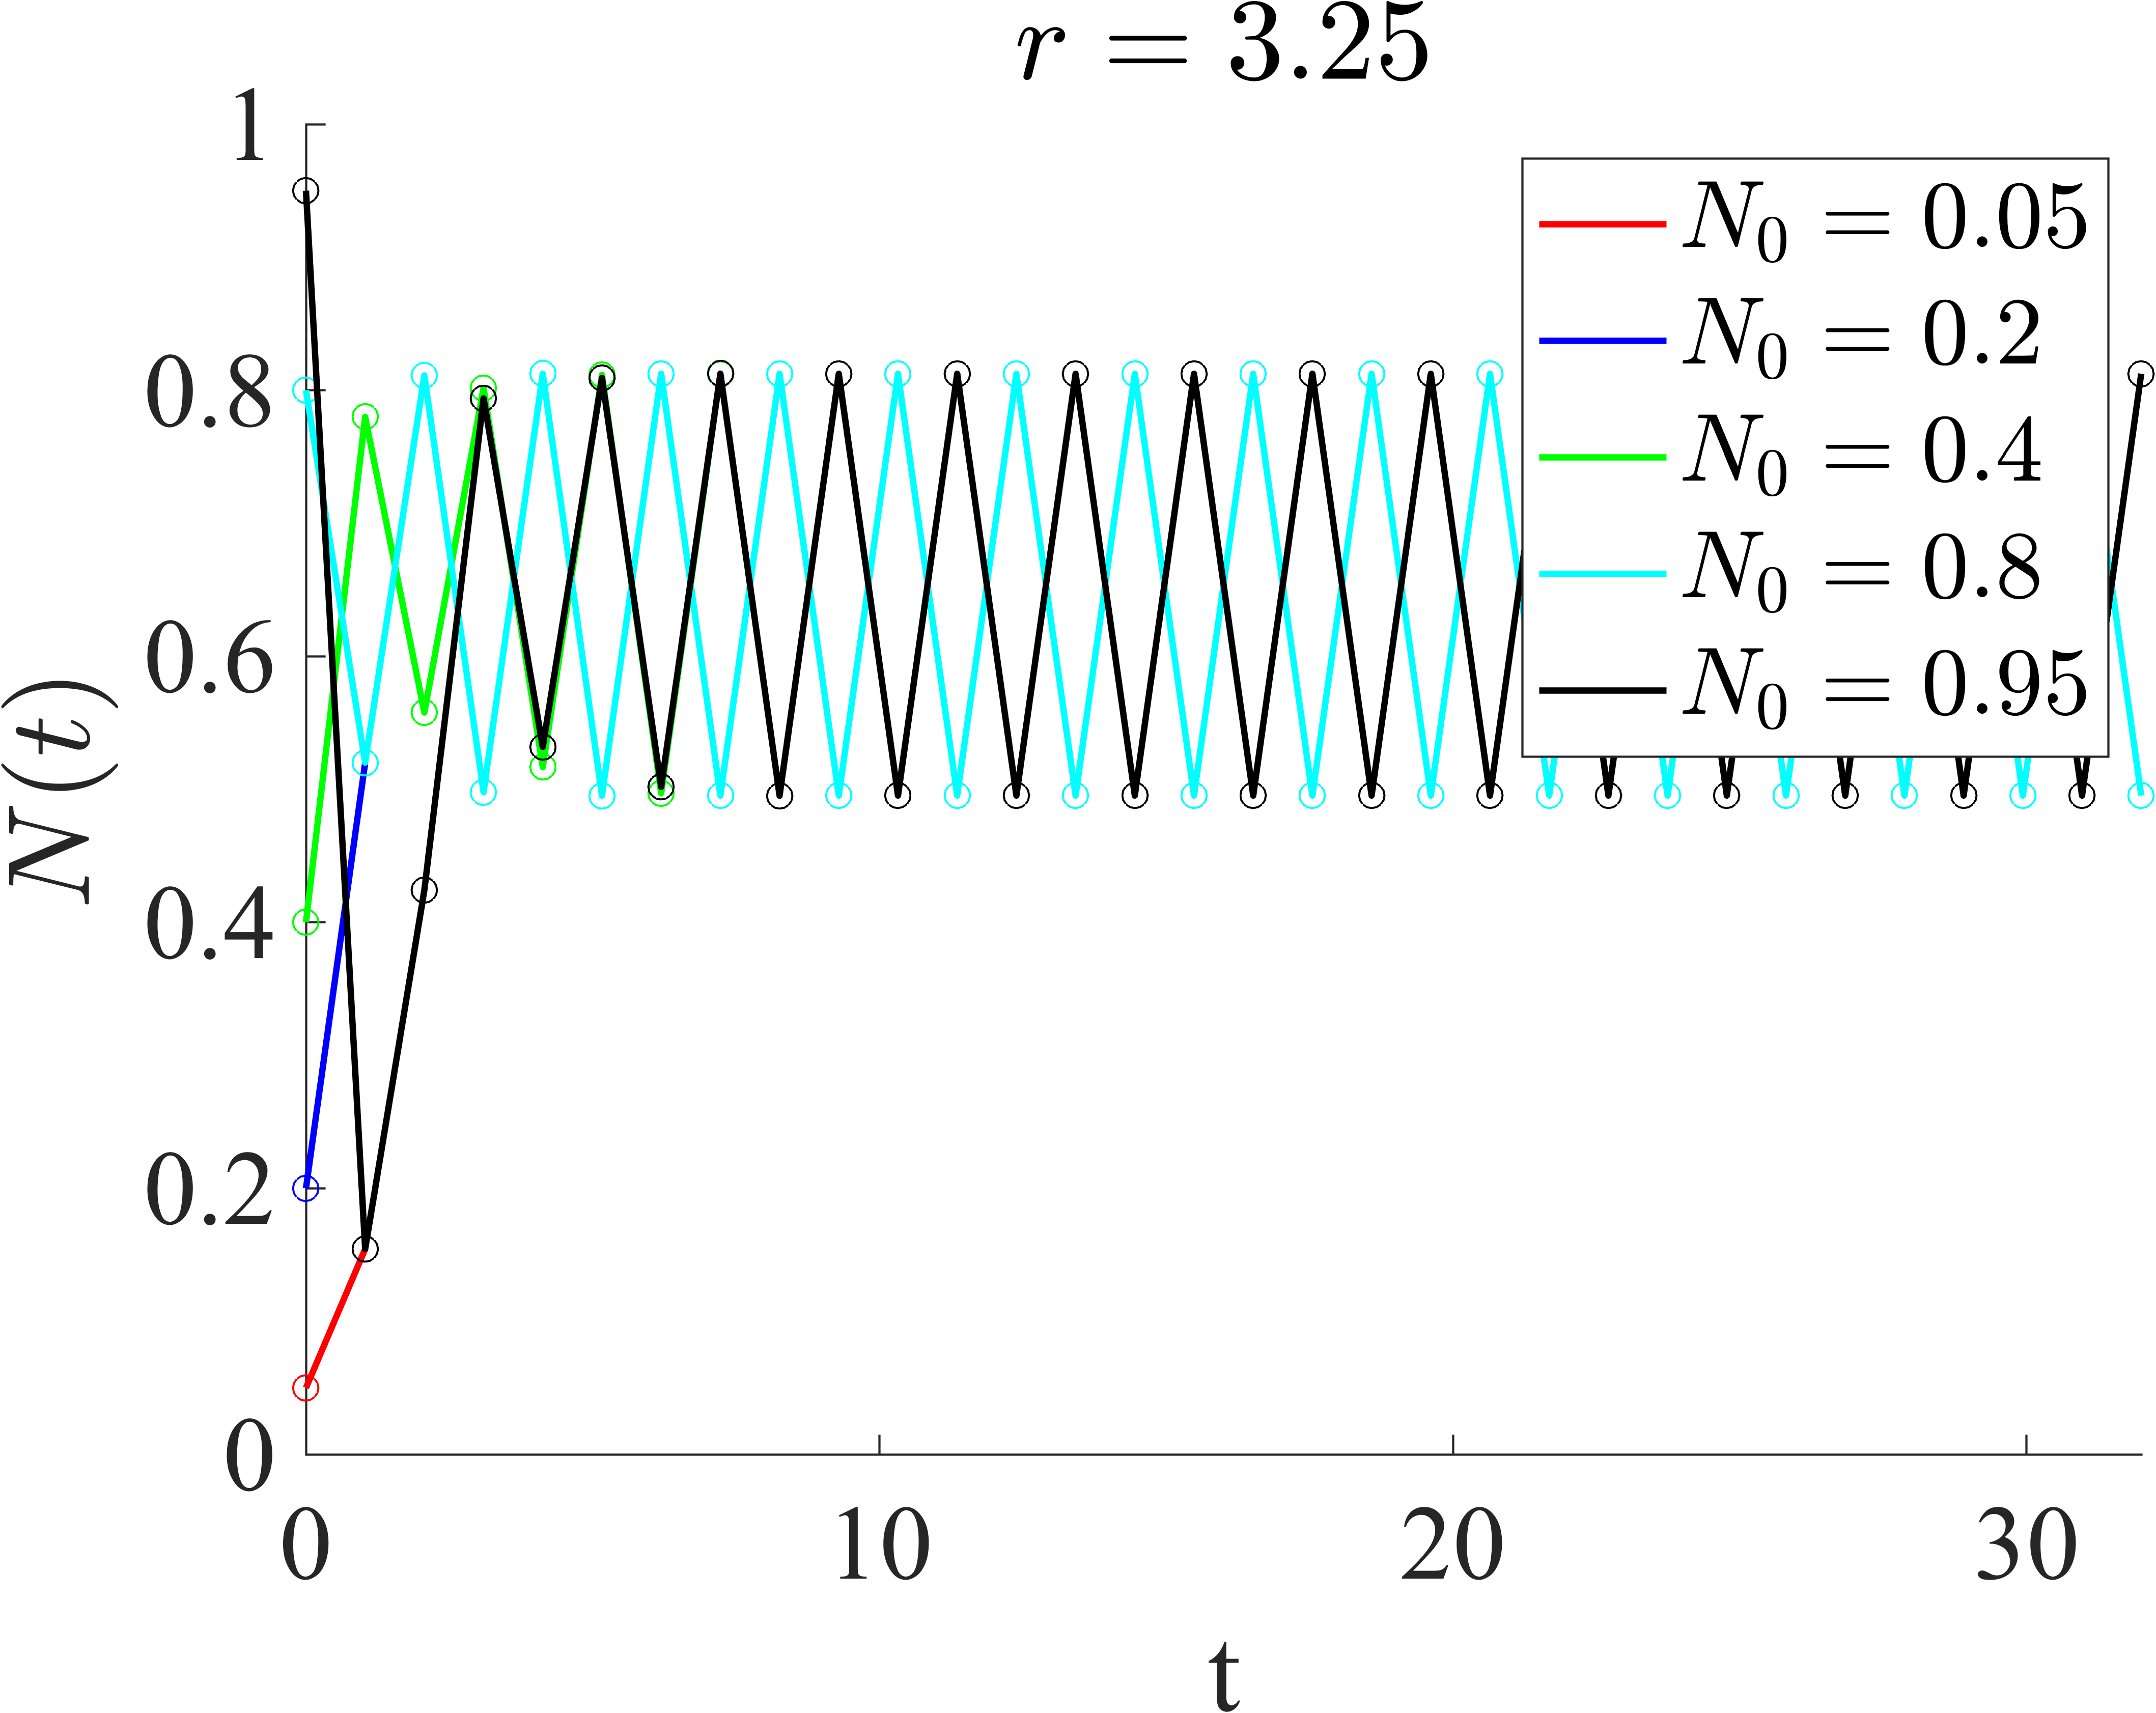
\includegraphics[width=10cm]{Logistic_map_r_3_25}
\caption{Logistic Map Solution Plot}
\end{figure}
With $r = 3.25$, the solutions appear to be in a stable oscillatory cycle of a period of 2 time steps.

\begin{figure}[H]
\centering
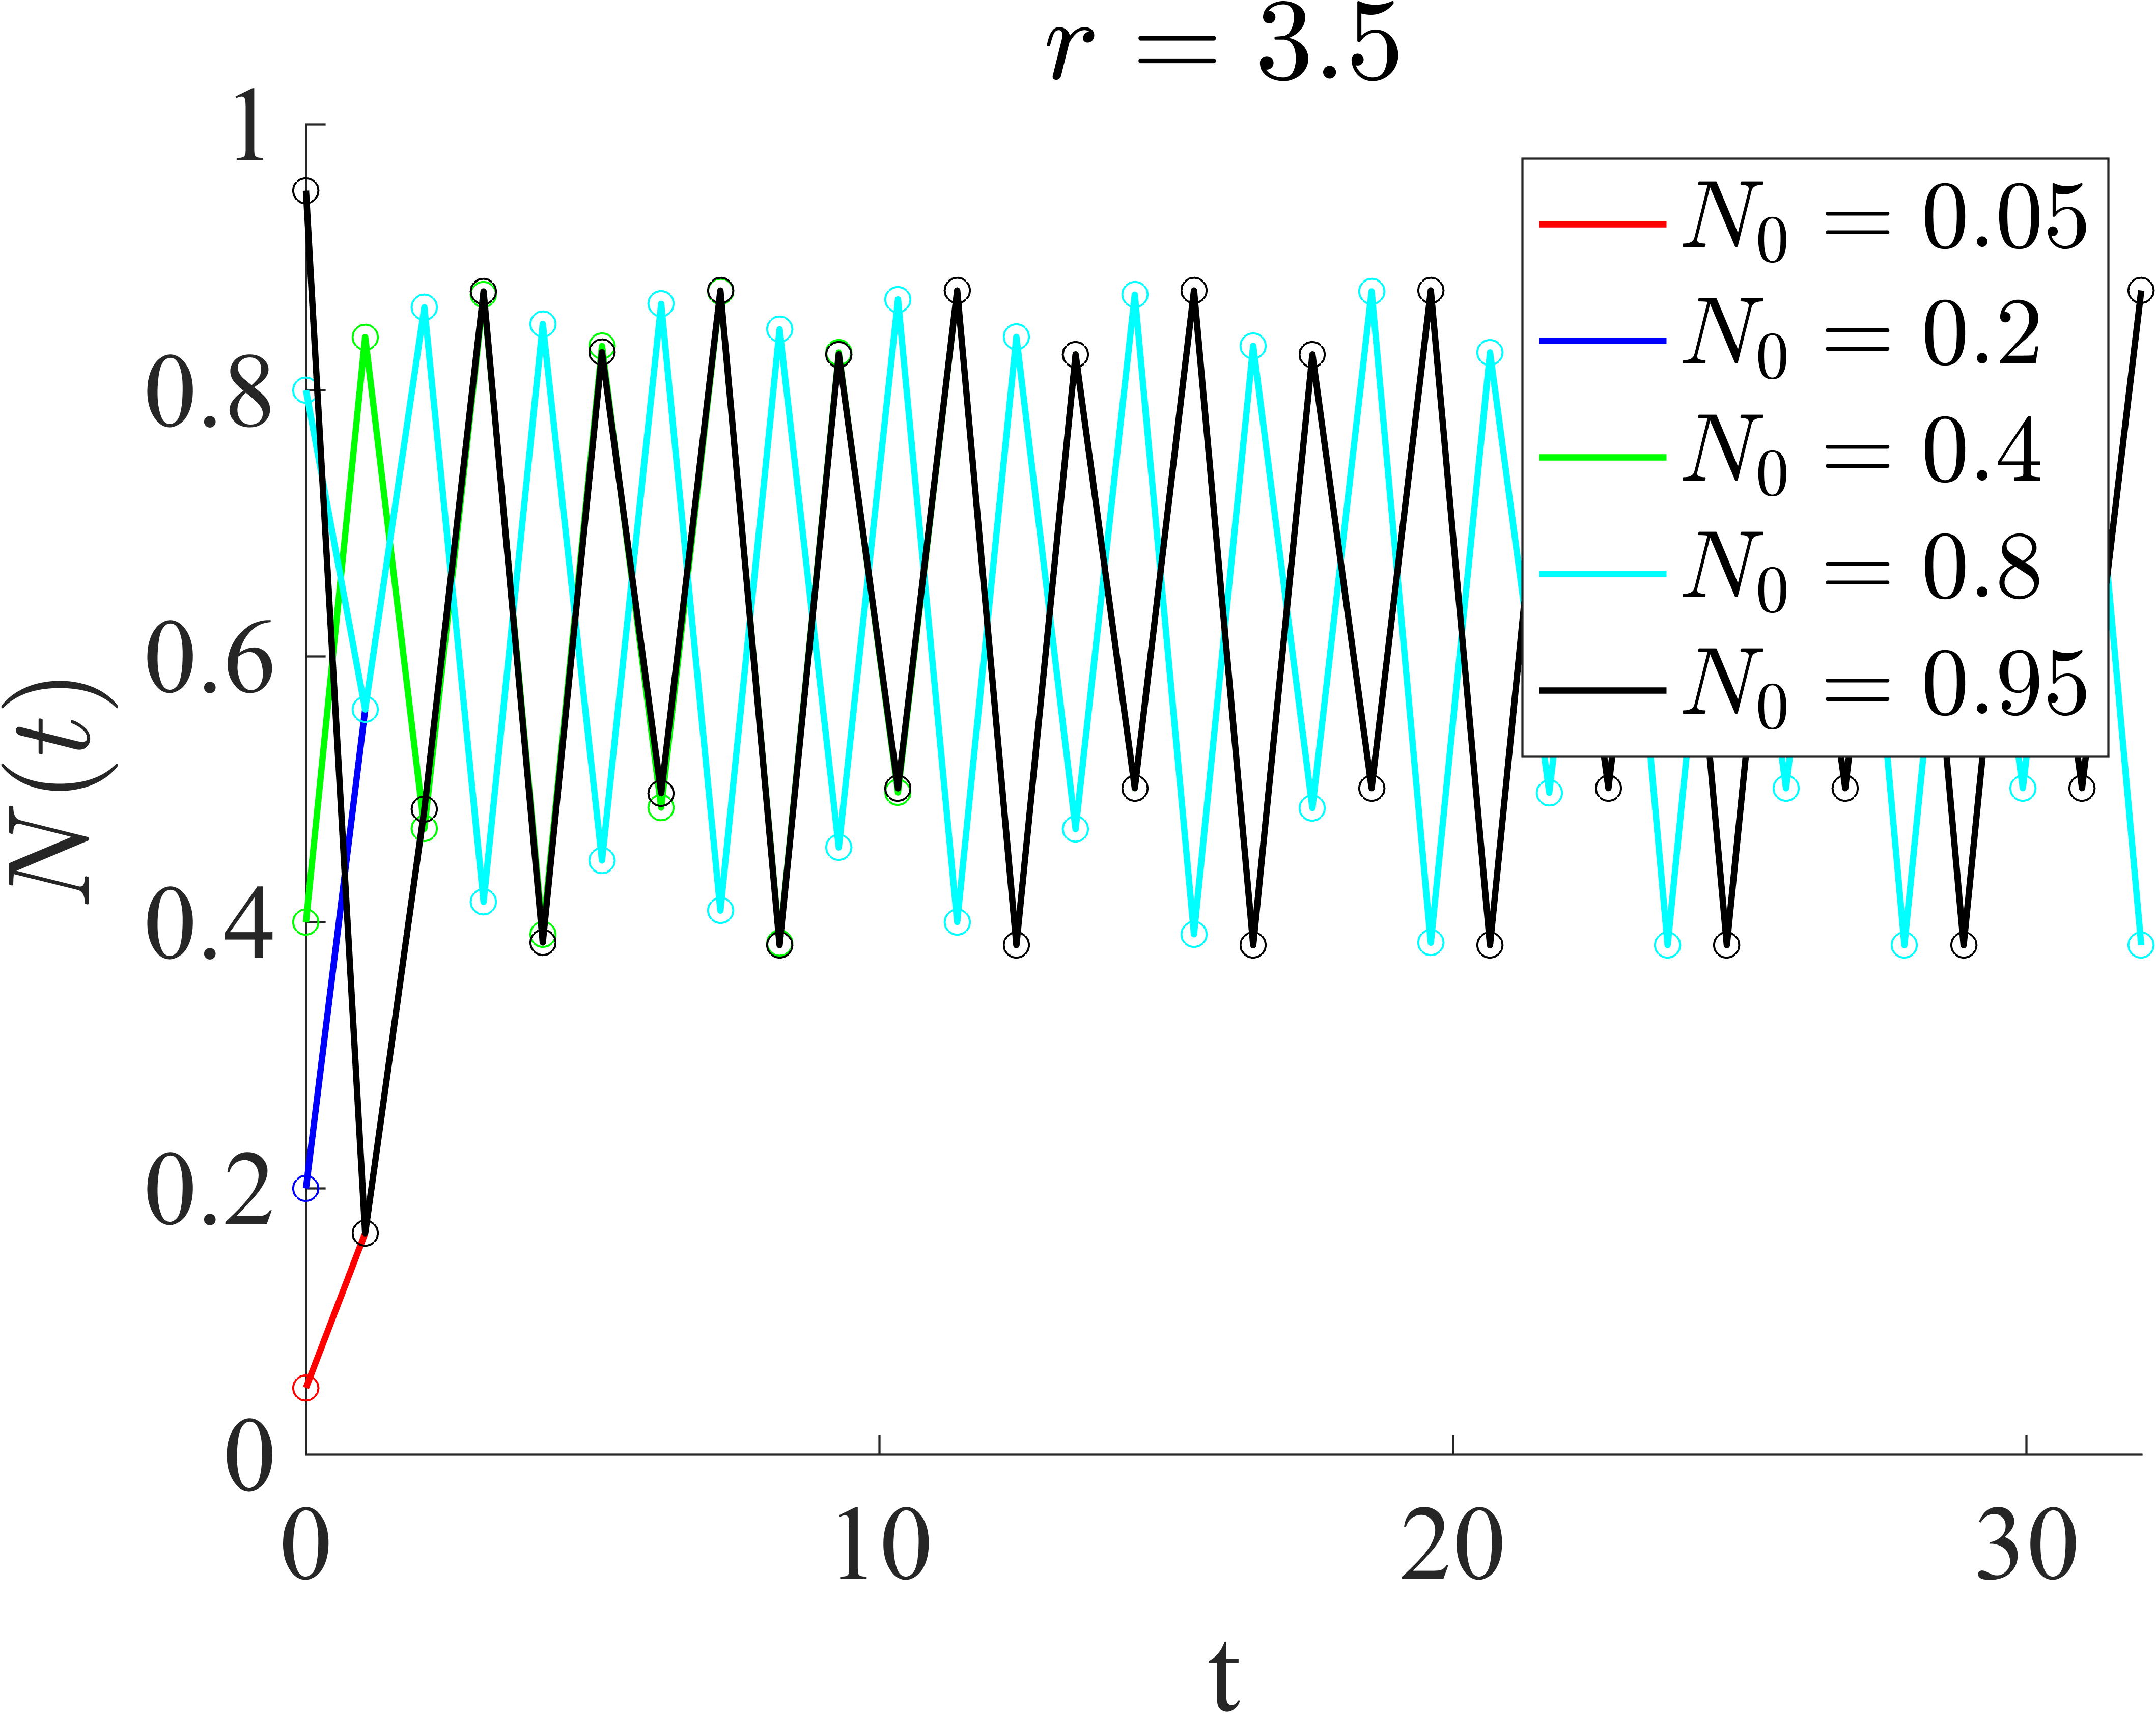
\includegraphics[width=10cm]{Logistic_map_r_3_5}
\caption{Logistic Map Solution Plot}
\end{figure}
With $r = 3.5$, the solutions appear to take on more complex oscillatory cycles of a period of 4 time steps.

\begin{figure}[H]
\centering
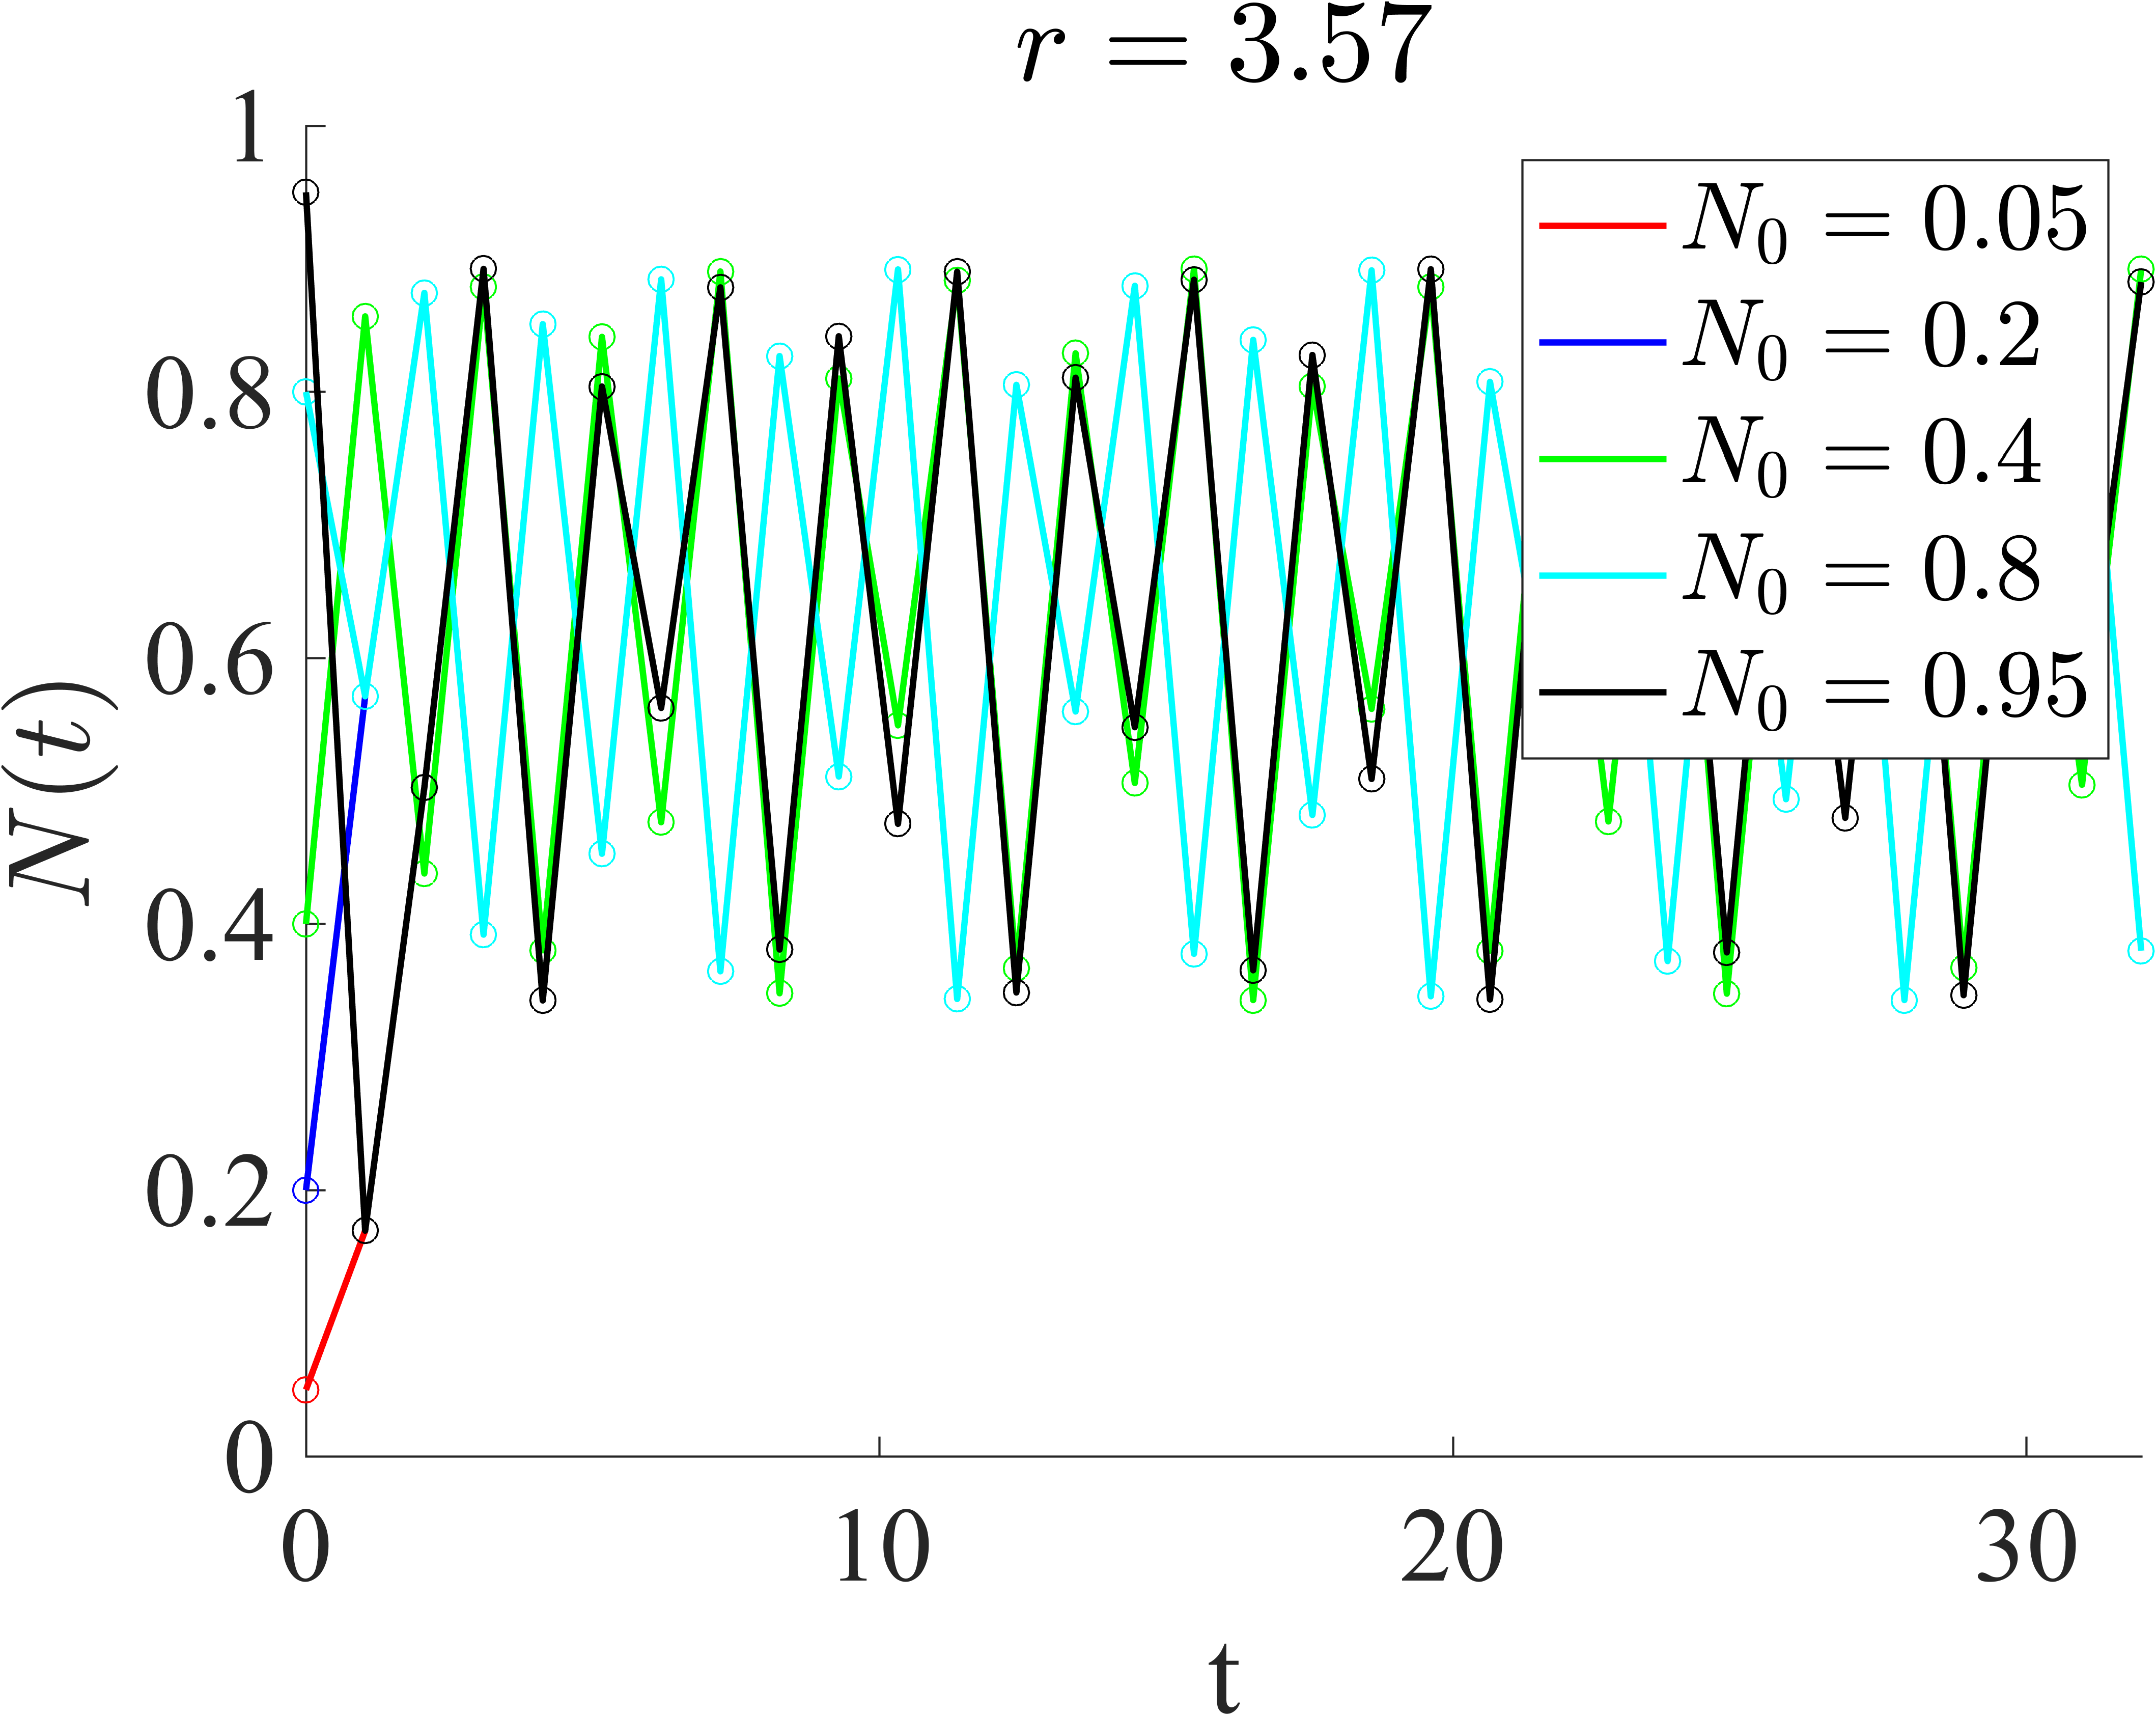
\includegraphics[width=10cm]{Logistic_map_r_3_57}
\caption{Logistic Map Solution Plot}
\end{figure}

With $r = 3.57$, the solutions now exhibit chaos and do not appear to have stable oscillations with a finite period. As previously stated, unlike discrete time equations, ODEs constrain the geometry of the flow because they are well-defined and finite throughout the entire state space $\Omega = [0,1]$. This means that the trajectories must be continuous and cannot cross. Furthermore, ODEs that are Lipschitz continuous also must have unique trajectories that cannot merge or branch in finite time.

\section*{Problem 9 Part 3}
I plot the function $f(\phi) = \frac{\omega}{4} \sqrt{4- sec(\phi(t))^2}$ below and plotted the derivative $\frac{d}{d\phi}$. We see in these figures below that the slope $\frac{d}{d\phi} f(\phi)$ diverges at  $\phi = \pm \frac{\pi}{3}$, implying that the solution trajectories are not unique. One could stay flying westward at a constant latitude of $60^{\circ}$ and choose to follow the optimal trajectory southward at any time. We can easily predict this non-uniqueness because the cusp of the function $f(\phi)$ at $\phi = \pm \frac{\pi}{3}$ tells us that the function is not Lipschitz continuous at those points, violating the uniqueness theorem. This means that there are exist finite trajectories traveling at $v_*$ that minimize the elapsed solar time. Trajectories can start at $\phi = \pm \frac{\pi}{3}$ and branch off at any time.

\begin{figure}[H]
\centering
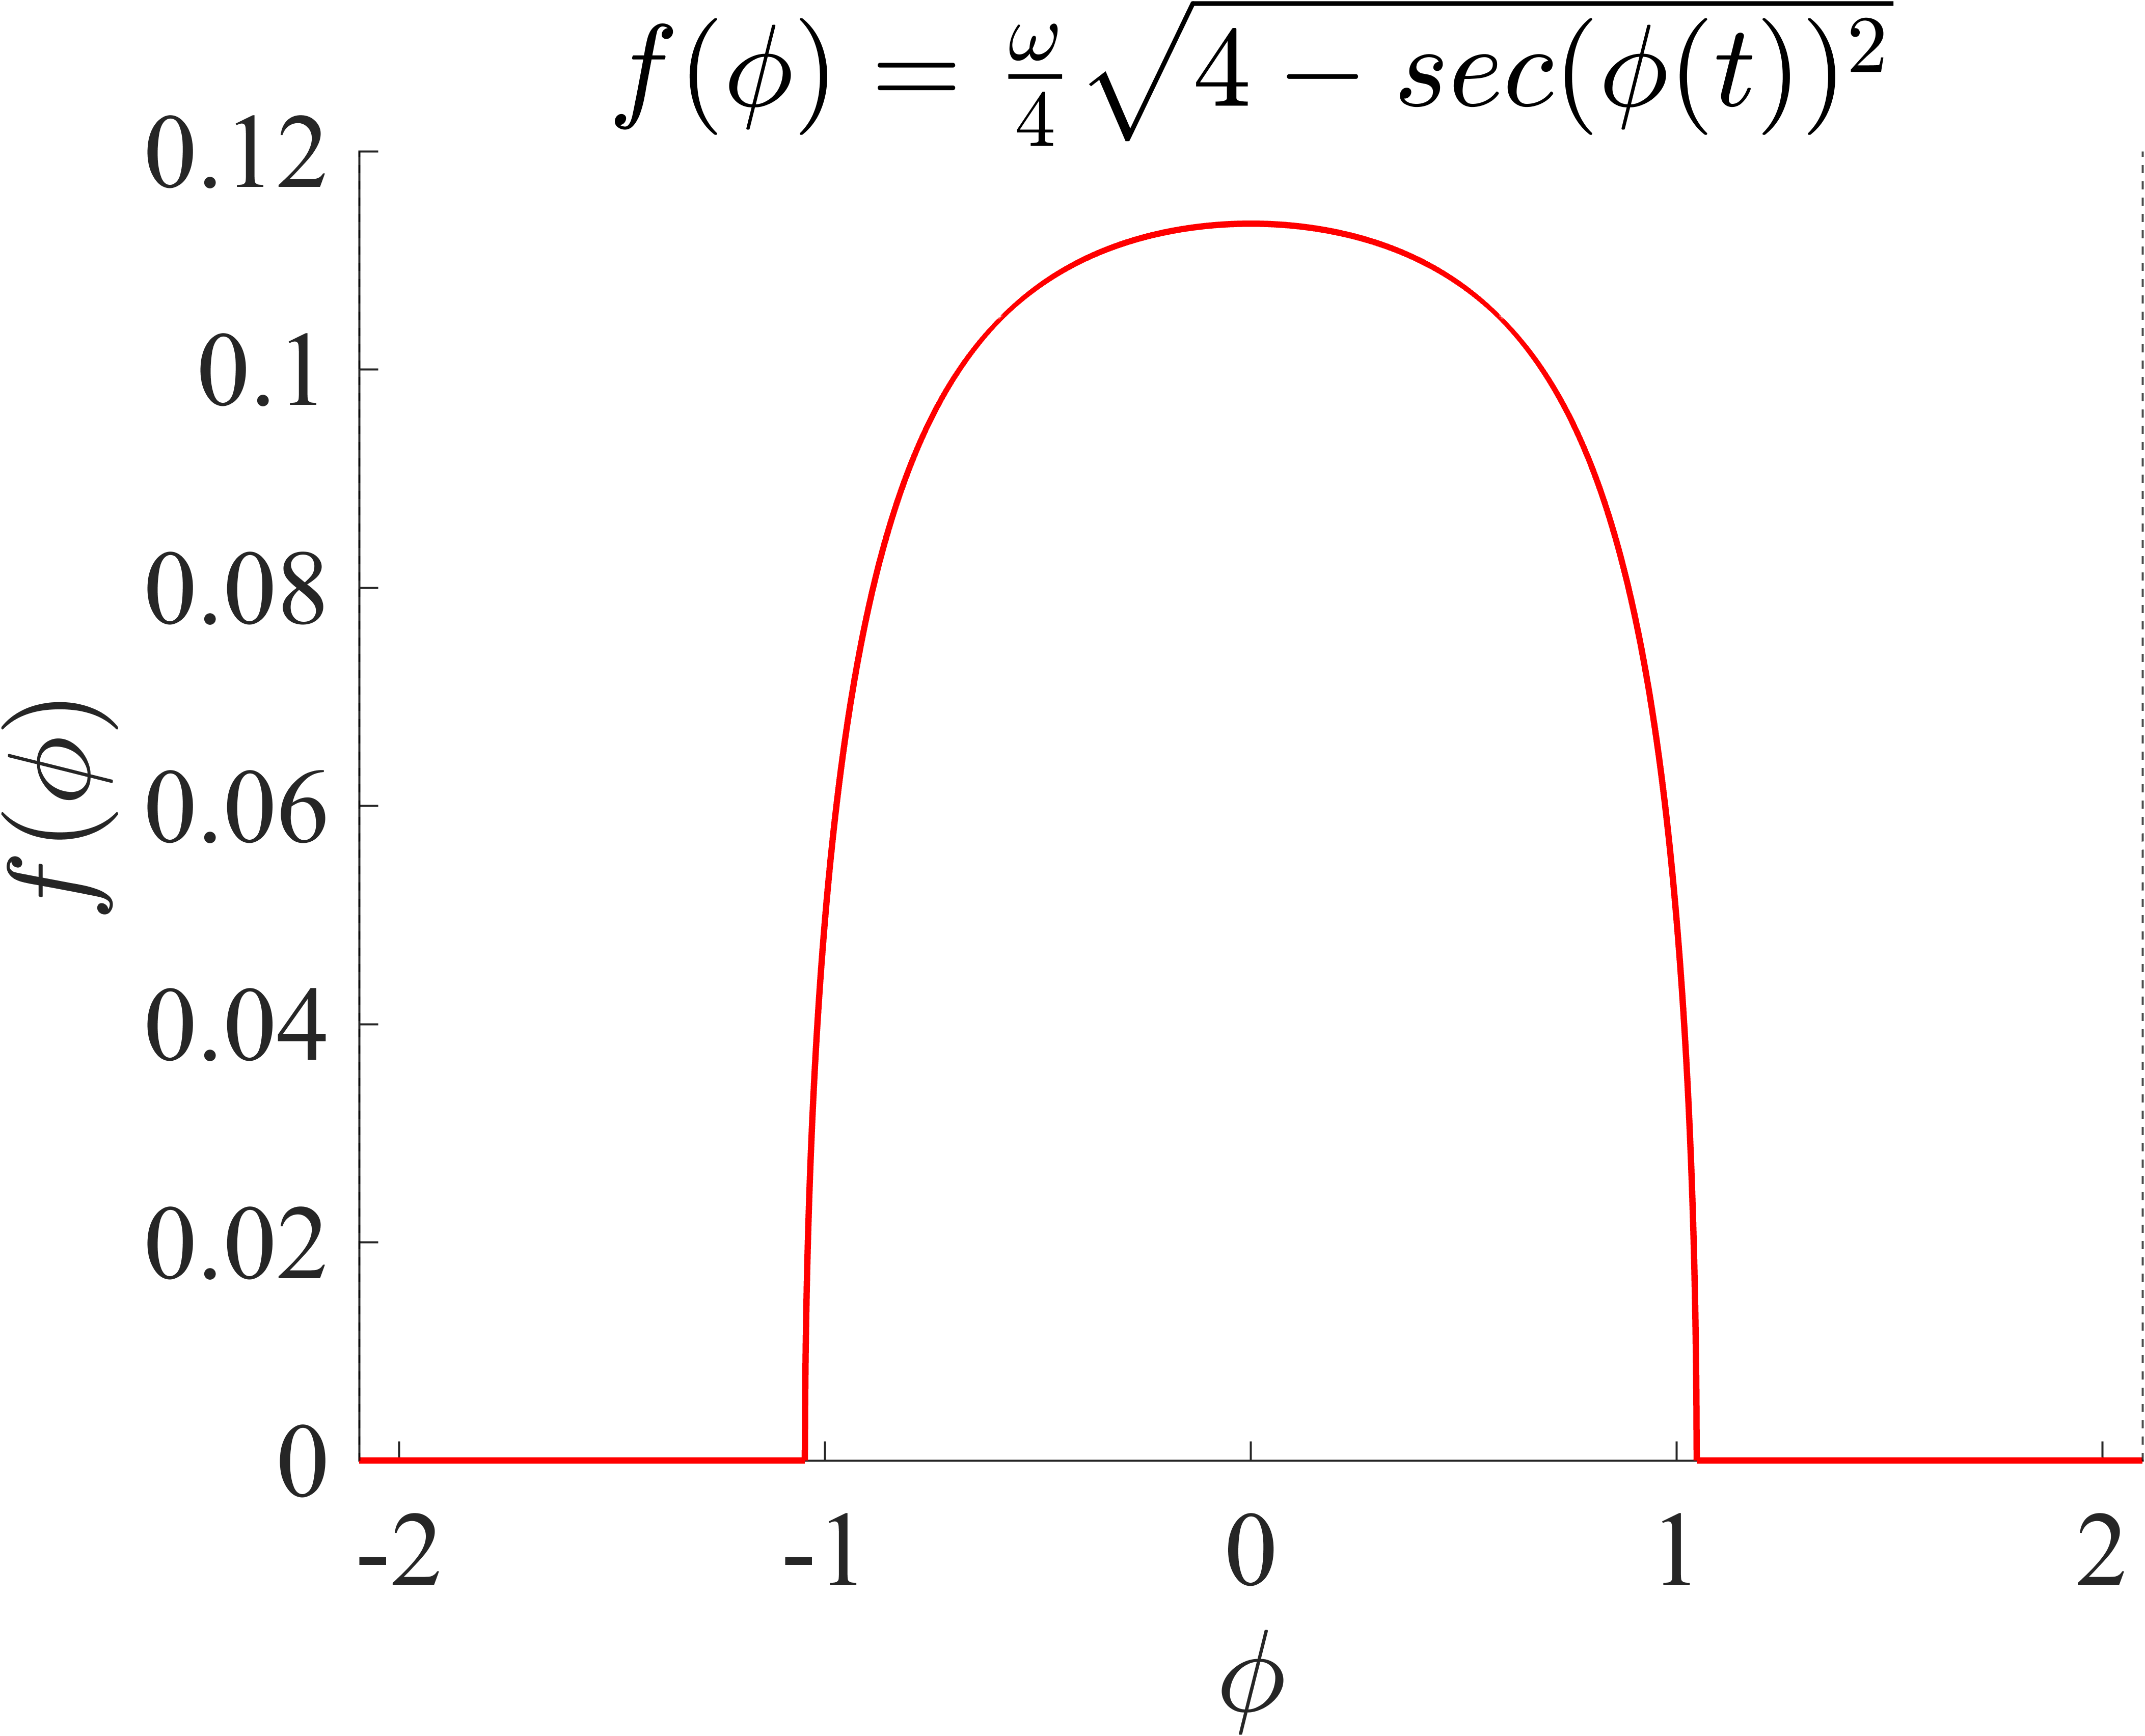
\includegraphics[width=.45\linewidth]{9_3}
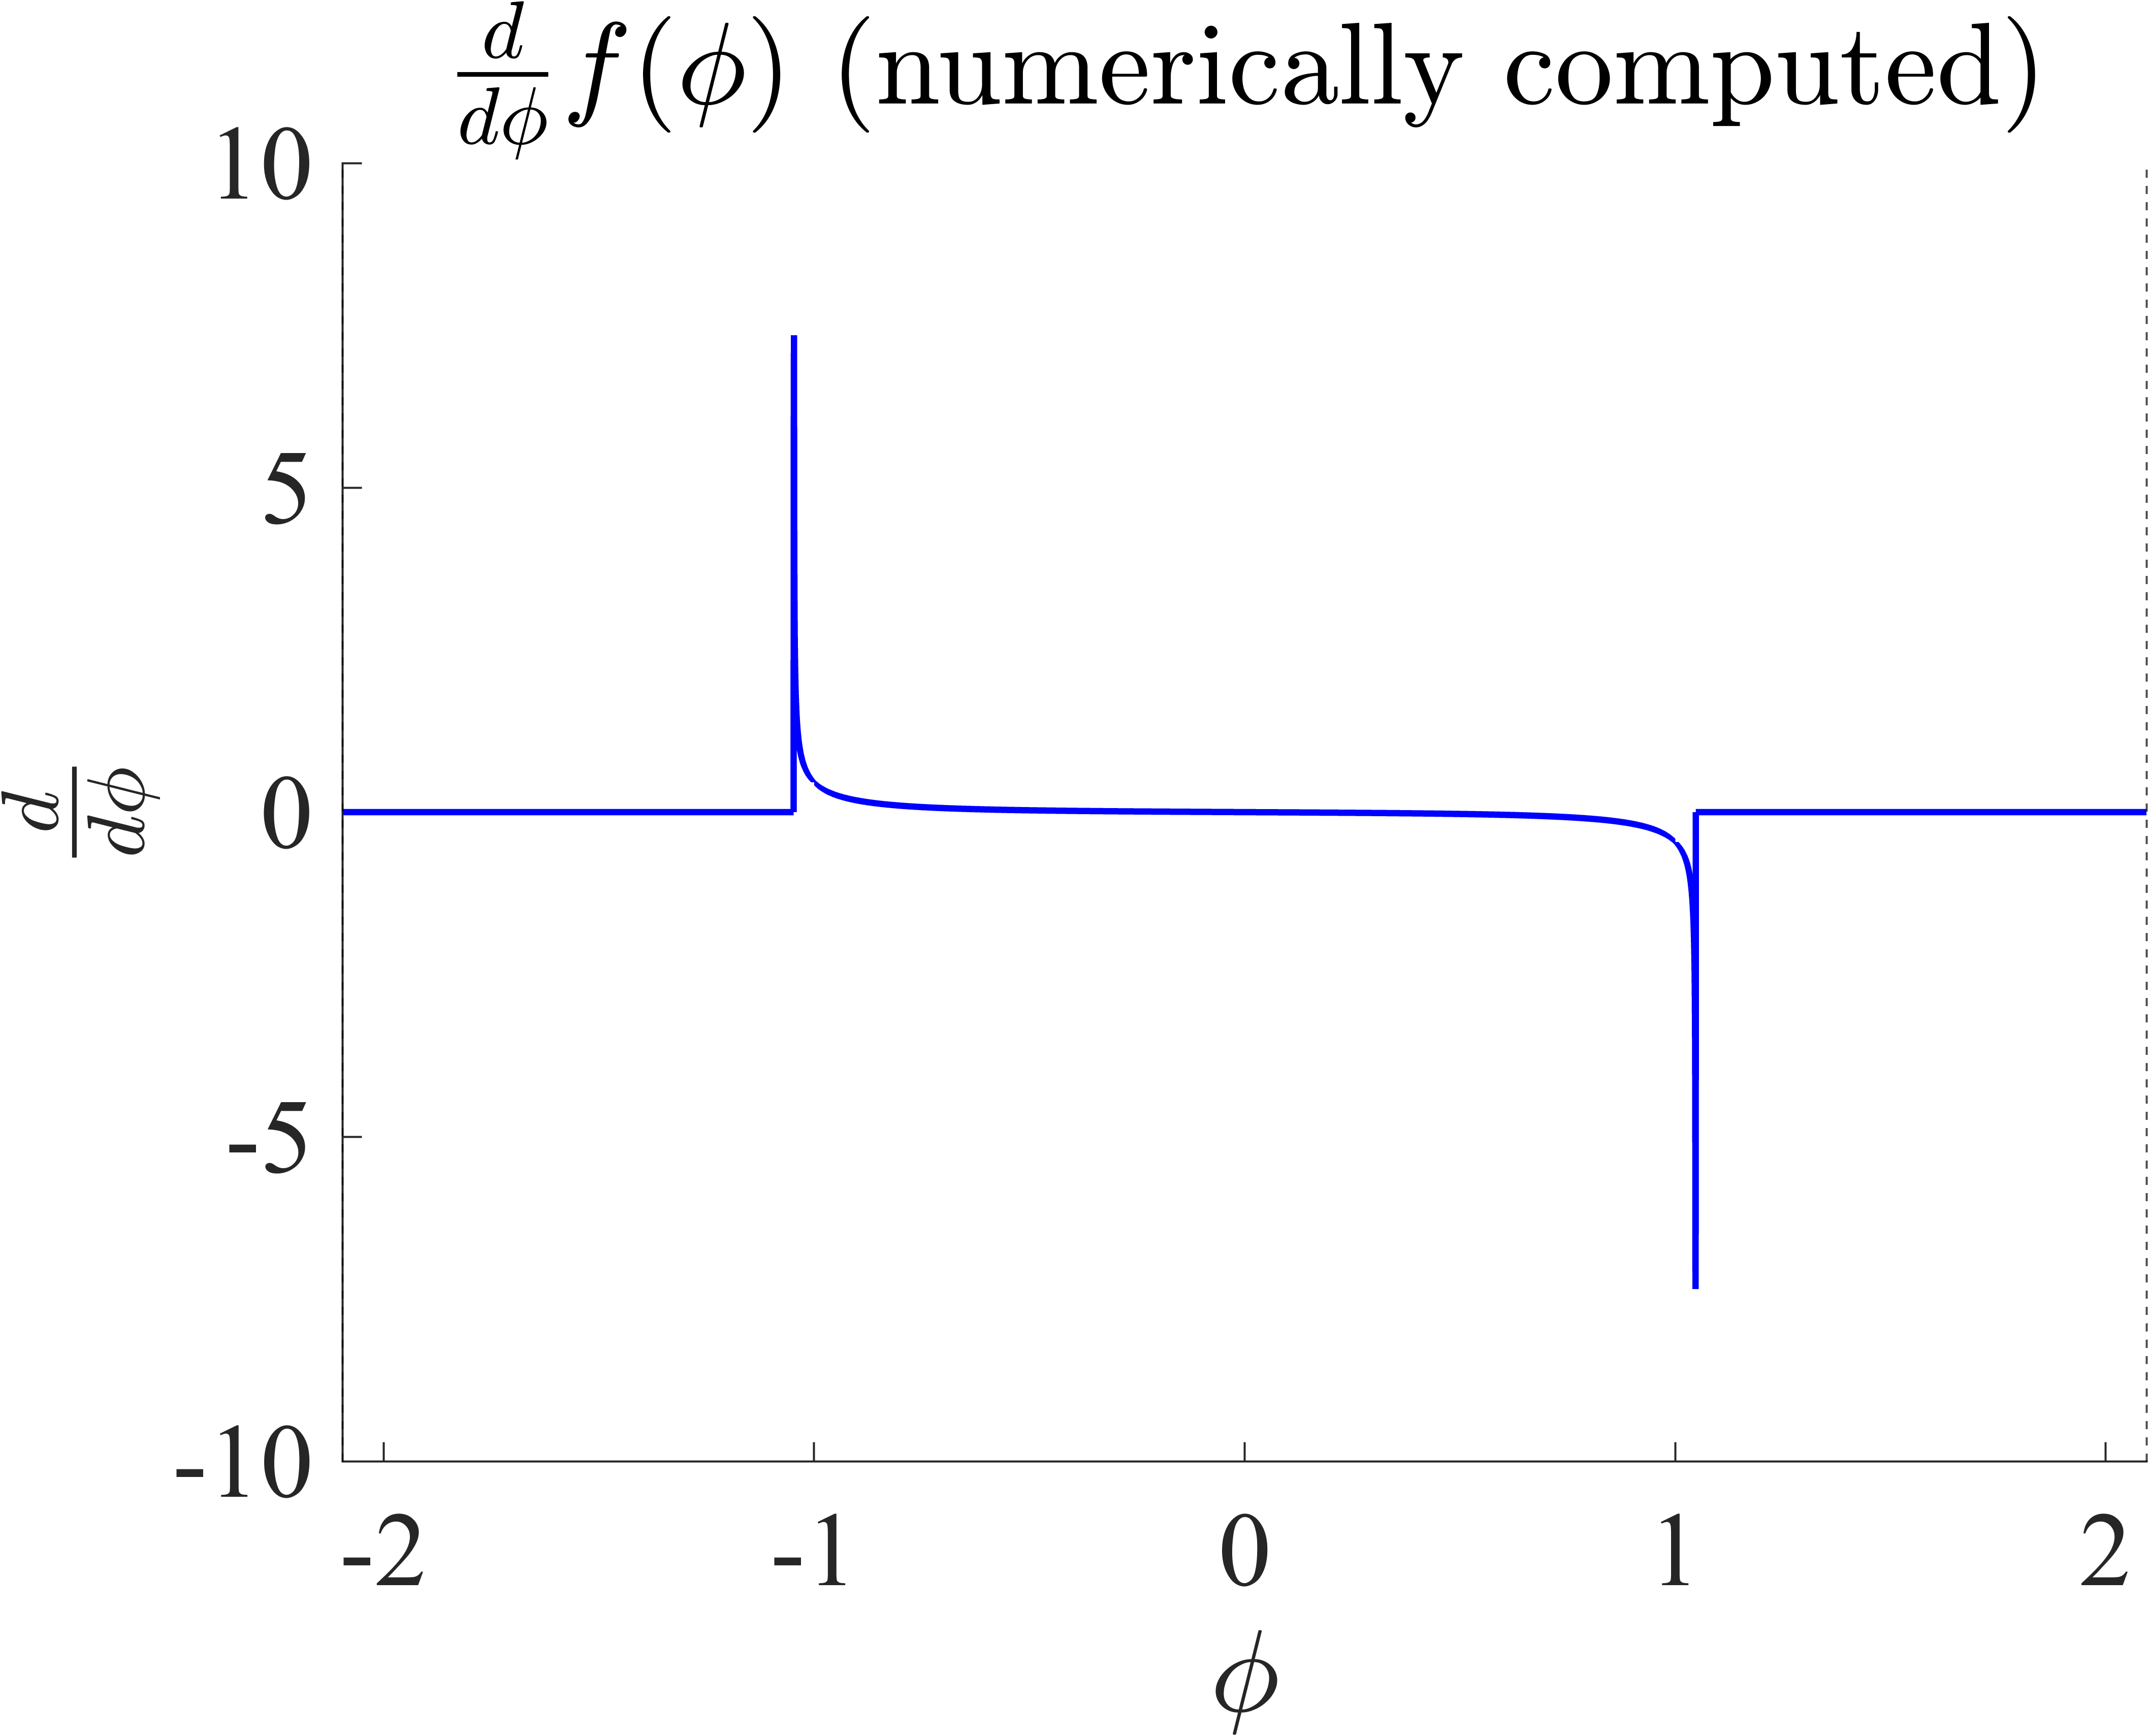
\includegraphics[width=.45\linewidth]{9_3_2}
\caption{Function Plot}
\end{figure}


\end{document}
